\documentclass[11pt, compress, t, notes = noshow, xcolor = table, 
aspectratio = 1610]{beamer}
\usepackage[]{graphicx}\usepackage[]{color}

\usepackage{framed}

\usepackage{alltt}
\newcommand{\SweaveOpts}[1]{}  % do not interfere with LaTeX
\newcommand{\SweaveInput}[1]{} % because they are not real TeX commands
\newcommand{\Sexpr}[1]{}       % will only be parsed by R

\usepackage[english]{babel}
\usepackage[utf8]{inputenc}
\usepackage{verbatim}
\usepackage{amsmath, nccmath}
\usepackage{amsfonts}
\usepackage{mathrsfs}
\usepackage{bm}
\usepackage{csquotes}
\usepackage{multirow}
\usepackage{longtable}
\usepackage{enumerate}
\usepackage[absolute,overlay]{textpos}
\usepackage{algorithm}
\usepackage{algpseudocode}
\usepackage{eqnarray}
\usepackage{arydshln}
\usepackage{tabularx}
\usepackage{setspace}
\usepackage{colortbl}
\usepackage{mathtools}
\usepackage{wrapfig}
\usepackage{bm}
\usepackage{xcolor}
\usepackage{caption}
\captionsetup[figure]{font=tiny}
\usepackage[labelformat=empty]{caption}
\usepackage{subcaption}
\usepackage[round, comma]{natbib}

% Defines macros and environments
% \usepackage{bbm}
% basic latex stuff
\newcommand{\pkg}[1]{{\fontseries{b}\selectfont #1}} %fontstyle for R packages
\newcommand{\lz}{\vspace{0.5cm}} %vertical space
\newcommand{\dlz}{\vspace{1cm}} %double vertical space
\newcommand{\oneliner}[1] % Oneliner for important statements
{\begin{block}{}\begin{center}\begin{Large}#1\end{Large}\end{center}\end{block}}


%new environments
\newenvironment{vbframe}  %frame with breaks and verbatim
{
 \begin{frame}[containsverbatim,allowframebreaks]
}
{
\end{frame}
}

\newenvironment{vframe}  %frame with verbatim without breaks (to avoid numbering one slided frames)
{
 \begin{frame}[containsverbatim]
}
{
\end{frame}
}

\newenvironment{blocki}[1]   % itemize block
{
 \begin{block}{#1}\begin{itemize}
}
{
\end{itemize}\end{block}
}

\newenvironment{fragileframe}[2]{  %fragile frame with framebreaks
\begin{frame}[allowframebreaks, fragile, environment = fragileframe]
\frametitle{#1}
#2}
{\end{frame}}


\newcommand{\myframe}[2]{  %short for frame with framebreaks
\begin{frame}[allowframebreaks]
\frametitle{#1}
#2
\end{frame}}

\newcommand{\remark}[1]{
  \textbf{Remark:} #1
}


\newenvironment{deleteframe}
{
\begingroup
\usebackgroundtemplate{
\includegraphics[width=\paperwidth,height=\paperheight]{../style/color/red.png}}
 \begin{frame}
}
{
\end{frame}
\endgroup
}
\newenvironment{simplifyframe}
{
\begingroup
\usebackgroundtemplate{
\includegraphics[width=\paperwidth,height=\paperheight]{../style/color/yellow.png}}
 \begin{frame}
}
{
\end{frame}
\endgroup
}\newenvironment{draftframe}
{
\begingroup
\usebackgroundtemplate{
\includegraphics[width=\paperwidth,height=\paperheight]{../style/color/green.jpg}}
 \begin{frame}
}
{
\end{frame}
\endgroup
}
% https://tex.stackexchange.com/a/261480: textcolor that works in mathmode
\makeatletter
\renewcommand*{\@textcolor}[3]{%
  \protect\leavevmode
  \begingroup
    \color#1{#2}#3%
  \endgroup
}
\makeatother

\usepackage{style/report}

% ------------------------------------------------------------------------------

\colorlet{highlightcol}{gray!90}
\newcommand{\maketag}[1]{\colorbox{highlightcol}{\textcolor{white}
{\MakeUppercase{#1}}}}
\newcommand{\highlight}[1]{\textcolor{highlightcol}{\textbf{#1}}}
\newcommand{\arritem}{\item[\highlight{$\rightarrow$}]}
\newcommand{\positem}{\item[$\highlight{+}$]}
\newcommand{\negitem}{\item[$\highlight{-}$]}
\newcommand{\flexitem}[1]{\item[$\highlight{#1}$]}
\newcommand{\conclbox}[1]{\fbox{\parbox{\textwidth}{\textbf{#1}}}}
\colorlet{GRAY}{gray}

\let\code=\texttt
\let\proglang=\textsf

\setkeys{Gin}{width=0.9\textwidth}

% ------------------------------------------------------------------------------

\newcommand{\topo}{\mathcal{T}}
\newcommand{\mani}{\mathcal{M}}
\newcommand{\N}{\mathbb{N}}
\newcommand{\R}{\mathbb{R}}
\newcommand{\RD}{\mathbb{R}^D}
\newcommand{\Rd}{\mathbb{R}^d}
\newcommand{\setN}{\{1, 2, ..., N\}}
\newcommand{\X}{\mathcal{X}}
\newcommand{\x}{\bm{x}}
\newcommand{\Y}{\mathcal{Y}}
\newcommand{\y}{\bm{y}}
\newcommand{\Ytil}{\tilde{\Y}}
\newcommand{\pv}{\bm{p}}
\newcommand{\qv}{\bm{q}}
\newcommand{\D}{\bm{D}}
\newcommand{\E}{\bm{E}}
\newcommand{\G}{\bm{G}}
\newcommand{\Hes}{\bm{H}}
\newcommand{\I}{\bm{I}}
\newcommand{\K}{\bm{K}}
\newcommand{\Lap}{\bm{L}}
\newcommand{\M}{\bm{M}}
\newcommand{\W}{\bm{W}}
\newcommand{\twonorm}[1]{\left\lVert #1 \right\rVert^2}
\newcommand{\frobnorm}[1]{\left\lVert #1 \right\rVert^2_F}

% ------------------------------------------------------------------------------

\title{Semi-Supervised Locally Linear Embedding (SSLLE)}
\author{Lisa Wimmer}
\date{February, 2021}

\setbeamertemplate{frametitle}{\expandafter\uppercase\expandafter
\insertframetitle}

\begin{document}

\lecturechapter{Application \& Sensitivity Analysis of Critical Parameters}
\lecture{Semi-Supervised Locally Linear Embedding (SSLLE)}

% ------------------------------------------------------------------------------
% AGENDA
% ------------------------------------------------------------------------------

\LARGE
\begin{frame}[noframenumbering]{\textcolor{gray!90}{0 agenda}}
\normalsize
\vspace{-0.5cm}
\noindent \textcolor{gray!90}{\rule{\textwidth}{1pt}}
\smallskip

\begin{itemize}
\large
\flexitem{1} Problem
\flexitem{2} Local graph-based manifold learning (LGML)
\flexitem{3} Techniques
\begin{itemize}
  \large
  \flexitem{1} Unsupervised
  \flexitem{2} Semi-supervised ~ \maketag{SSLLE}
  \flexitem{3} Challenges
\end{itemize}
\flexitem{4} Sensitivity analysis
\begin{itemize}
  \large
  \flexitem{1} Setup
  \flexitem{2} Results
\end{itemize}
\flexitem{5} Discussion
\end{itemize}

\end{frame}

% ------------------------------------------------------------------------------
% MANIFOLD LEARNING PROBLEM
% ------------------------------------------------------------------------------

\LARGE
\begin{frame}{\textcolor{gray!90}{1 problem} ~~ manifold learning}
\normalsize
\vspace{-0.5cm}
\noindent \textcolor{gray!90}{\rule{\textwidth}{1pt}}
\smallskip

\textbf{Situation:} rapidly increasing amount of data thanks to novel 
applications and data sources

\vspace{0.5cm}

\begin{minipage}[b]{0.7\textwidth}
  \raggedright
  \textbf{Problem:} high data dimensionality detrimental to
  \begin{itemize}
    \flexitem{1} model functionality
    \flexitem{2} interpretability
    % \arritem Generalization ability
  \end{itemize}
  \medskip
  \textbf{Manifold assumption:} data in high-dimensional observation
  space truly sampled from low-dimensional manifold
\end{minipage}%
\begin{minipage}[b]{0.3\textwidth}
  \begin{figure}[H]
    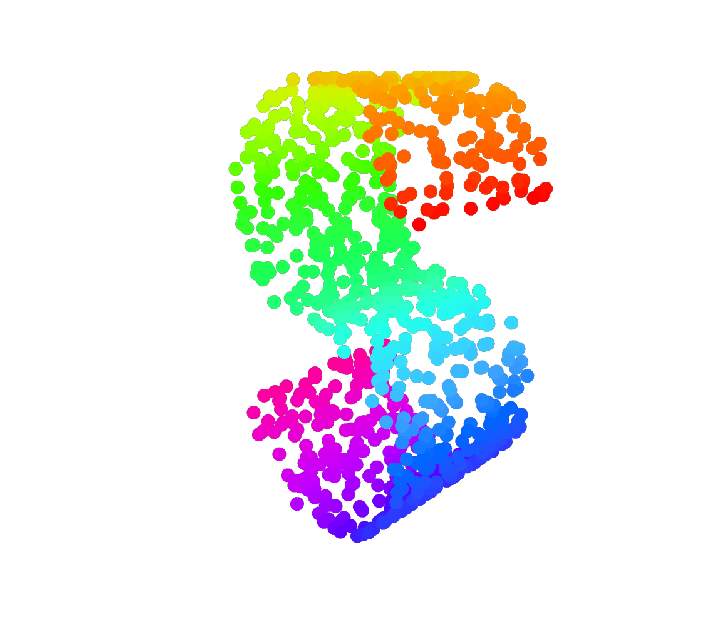
\includegraphics[trim = 70 40 70 30, clip, % left bottom right top
      width = 0.55\textwidth]{figures/s_curve}
  \end{figure}
\end{minipage}

\vfill

\conclbox{How to find a meaningful, structure-preserving embedding?}

\end{frame}

\LARGE
\begin{frame}{\textcolor{gray!90}{1 problem} ~~ manifold learning}
\normalsize
\vspace{-0.5cm}
\noindent \textcolor{gray!90}{\rule{\textwidth}{1pt}}
\smallskip

\textbf{Formal goal of manifold learning:}
\medskip
\begin{itemize}
  \arritem \textbf{Given:} data $\X = (\x_1, \x_2, ..., \x_N)$, with $\x_i \in 
  \RD$ $\forall i \in \setN$ and $N, D \in \N$, supposedly lying on 
  $d$-dimensional manifold $\mani$ \\
  $\Rightarrow$ $\psi: \mani \rightarrow \Rd$ with $d \ll D, d \in \N$ \\
  $\Rightarrow$ $\X \sim \mani \subset \RD$ 
  \medskip
  \arritem \textbf{Goal:} find $d$-dimensional Euclidean representation \\
  $\Rightarrow$ $\Y = (\y_1, \y_2, ..., \y_N)$, with 
  $\y_i = \psi(\x_i) \in \R^d$ $\forall i \in \setN$.
\end{itemize}

\vfill

\begin{figure}[H]
 \begin{subfigure}[c]{0.2\textwidth}
  \centering
   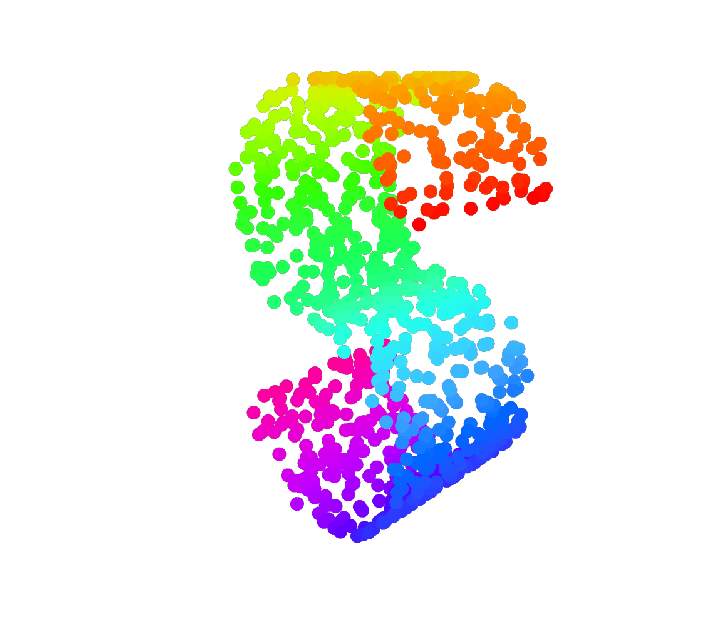
\includegraphics[trim = 70 30 70 30, clip, % left bottom right top
      width = 0.63\textwidth]{figures/s_curve}
 \end{subfigure}
 \hfill
 \begin{subfigure}[c]{0.7\textwidth}
   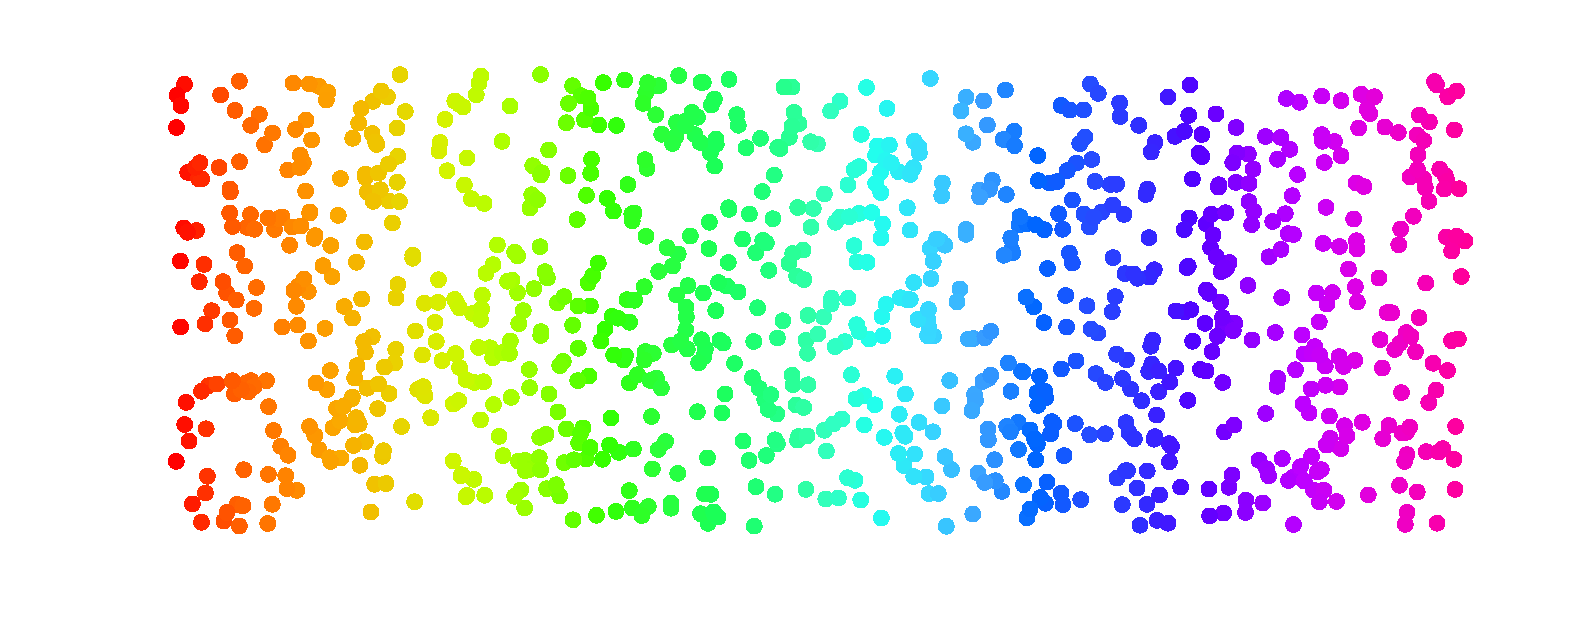
\includegraphics[trim = 80 20 0 0, clip, % left bottom right top
      width = 0.6\textwidth]{figures/s_curve_undone}
 \end{subfigure}
\end{figure}

\end{frame}

% ------------------------------------------------------------------------------
% LGML
% ------------------------------------------------------------------------------

\LARGE
\begin{frame}[noframenumbering]{\phantom{foo}}
\normalsize
\vspace{-0.5cm}
\noindent \textcolor{gray!90}{\rule{\textwidth}{1pt}}
\smallskip

\Huge
\hspace{0pt}
\vfill
\textbf{\highlight{~~ 2 ~~ LGML}}
\vfill
\hspace{0pt}

\noindent \textcolor{gray!90}{\rule{\textwidth}{1pt}}

\end{frame}

% ------------------------------------------------------------------------------

\LARGE
\begin{frame}{\textcolor{gray!90}{2 lgml} ~~ taxonomy}
\normalsize
\vspace{-0.5cm}
\noindent \textcolor{gray!90}{\rule{\textwidth}{1pt}}
\smallskip

\textbf{Landscape:} various approaches, many of which may be translated into one
another

\vspace{0.5cm}

\begin{minipage}[b]{0.65\textwidth}
  \begin{figure}[H]
    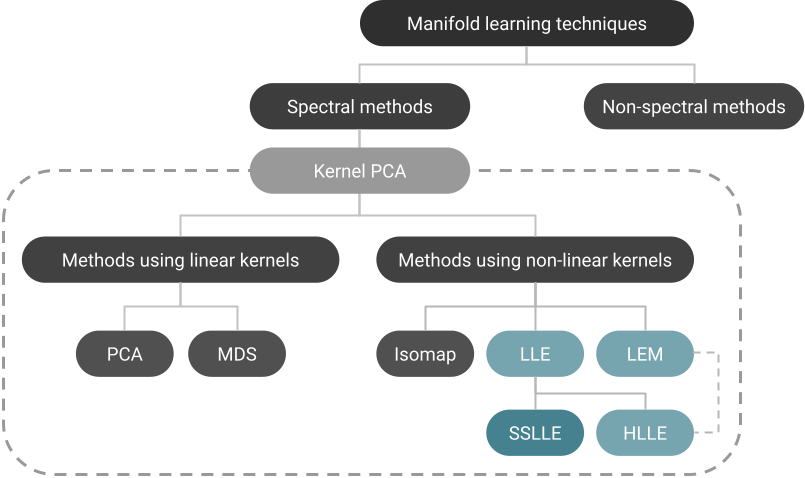
\includegraphics[trim = 0 0 0 0, clip, % left bottom right top
      width = \textwidth]{figures/models_overview}
  \end{figure}
\end{minipage}%
\begin{minipage}[b]{0.35\textwidth}
  \highlight{LEM} ~ Laplacian eigenmaps \\
  \highlight{LLE} ~ locally linear embedding \\
  \highlight{HLLE} ~ Hessian LLE \\
  \highlight{SSLLE} ~ semi-supervised LLE 
\end{minipage}

\end{frame}

% ------------------------------------------------------------------------------

\LARGE
\begin{frame}{\textcolor{gray!90}{2 lgml} ~~ concept}
\normalsize
\vspace{-0.5cm}
\noindent \textcolor{gray!90}{\rule{\textwidth}{1pt}}
\smallskip

\textbf{Idea:} capture intrinsic geometry, find principal axes of variability, 
retain most salient ones

\medskip

\begin{figure}[H]
  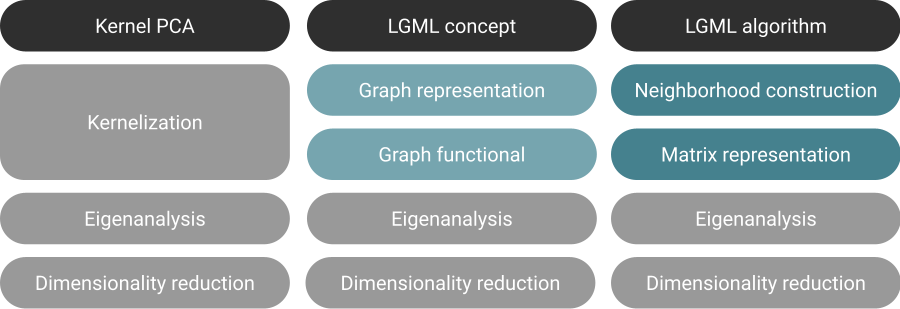
\includegraphics[trim = 0 0 0 0, clip, % left bottom right top
    width = \textwidth]{figures/kpca_lgml_algo}
\end{figure}

\vfill

\conclbox{Achievements: non-linearity \& locality}

\end{frame}

% ------------------------------------------------------------------------------

\LARGE
\begin{frame}{\textcolor{gray!90}{2 lgml} ~~ concept}
\normalsize
\vspace{-0.5cm}
\noindent \textcolor{gray!90}{\rule{\textwidth}{1pt}}
\smallskip

\textbf{Graph representation:} constructing a skeletal model of the manifold in 
$\RD$

\vspace{0.3cm}

\begin{minipage}[b]{0.67\textwidth}
  \medskip
  \textbf{Vertices:} given by observations \\
  \textbf{Edges:} present between neighboring points
    \begin{itemize} 
      \arritem Typically, $k$-neighborhoods
      \arritem Edge weights determined by nearness
    \end{itemize}
  \vspace{0.3cm}
  \textbf{Graph functional:} belief about intrinsic manifold properties at the 
  heart of each method
  \begin{itemize}
    \arritem Smoothness ~ \maketag{LEM}
    \arritem Curviness ~ \maketag{HLLE}
    \arritem Local linearity ~ \maketag{LLE} \maketag{SSLLE}
  \end{itemize}
\end{minipage}%
\begin{minipage}[b]{0.33\textwidth}
  \begin{figure}[H]
    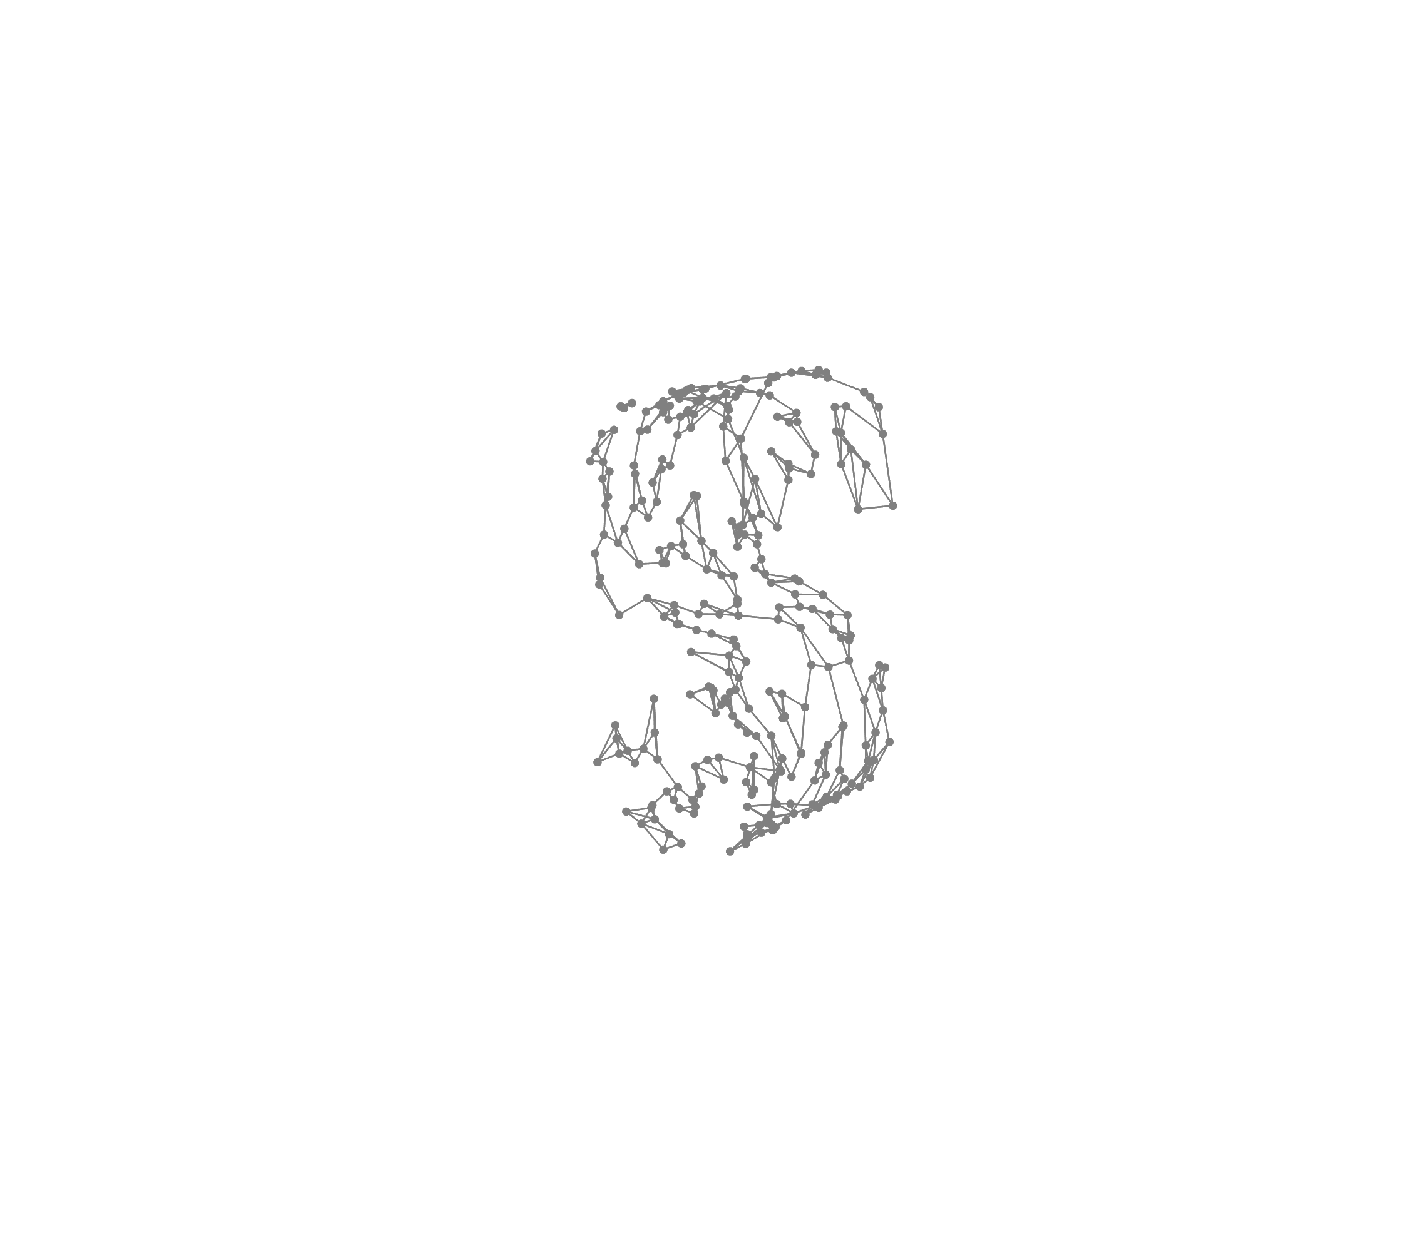
\includegraphics[trim = 250 190 220 160, clip, % left bottom right top
      width = 0.9\textwidth]{figures/s_curve_connected}
  \end{figure}
\end{minipage}

\end{frame}

% ------------------------------------------------------------------------------

\LARGE
\begin{frame}<presentation:0>[noframenumbering]
{\textcolor{gray!90}{2 lgml} ~~ concept}
\normalsize
\vspace{-0.5cm}
\noindent \textcolor{gray!90}{\rule{\textwidth}{1pt}}
\smallskip

\textbf{Eigenanalysis:} finding axes of variability in intrinsic 
manifold structure

\begin{itemize}
  \arritem Matrix representation of manifold properties
  \arritem Assessment through eigenanalysis
  \begin{itemize}
    \arritem Directions of variability $\Rightarrow$ eigenvectors
    \arritem Respective degrees of variability $\Rightarrow$ eigenvalues
  \end{itemize}
\end{itemize}

\vspace{0.3cm}

\textbf{Dimensionality reduction:} projection into subspace 
spanned by $d$ principal eigenvectors

\vspace{0.3cm}

\begin{figure}[H]
  \raggedright
  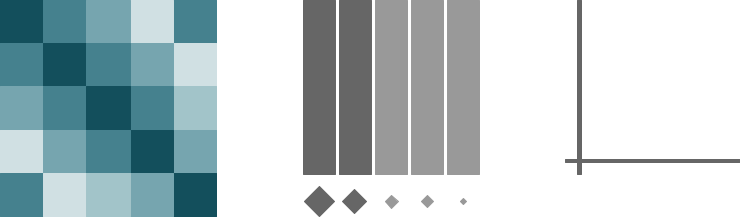
\includegraphics[trim = 0 0 0 0, clip, % left bottom right top
    width = 0.6\textwidth]{figures/eigenanalysis}
\end{figure}

\end{frame}

% ------------------------------------------------------------------------------
% LGML TECHNIQUES
% ------------------------------------------------------------------------------

\LARGE
\begin{frame}[noframenumbering]{\phantom{foo}}
\normalsize
\vspace{-0.5cm}
\noindent \textcolor{gray!90}{\rule{\textwidth}{1pt}}
\smallskip

\Huge
\hspace{0pt}
\vfill
\textbf{\highlight{~~ 3 ~~ TECHNIQUES}}
\vfill
\hspace{0pt}

\noindent \textcolor{gray!90}{\rule{\textwidth}{1pt}}

\end{frame}

% ------------------------------------------------------------------------------

\LARGE
\begin{frame}%<presentation:0>[noframenumbering]
{\textcolor{gray!90}{3.1 unsupervised} ~~ lem}

\normalsize
\vspace{-0.5cm}
\noindent \textcolor{gray!90}{\rule{\textwidth}{1pt}}
\smallskip

\textbf{Proposal:} \citet{belkinniyogi2001}

\vspace{0.3cm}

\textbf{Idea:} forcing nearby inputs to be mapped to nearby outputs

\begin{itemize}
  \arritem Notion of smoothness in mapping function
  \arritem Second-order penalty on gradient
\end{itemize}

\vspace{0.3cm}

\textbf{Solution:} eigenanalysis of graph Laplacian $\Lap$

\begin{itemize}
  \arritem Derived from weight matrix encoding nearness of inputs
  \arritem Discrete approximation of Laplace-Beltrami operator $\mathcal{L}(f)$
  \arritem Generalized eigenvalue problem
\end{itemize}

% \textbf{Graph Laplacian}. Discrete approximation of Laplace-Beltrami operator
% 
% \begin{itemize}
%   \arritem Weight matrix. $\W = (w)_{ij} \in \R^{N \times N}$, where 
%   $w_{ij} = w_{ij}(\twonorm{\x_i - \x_j})$
%   % \arritem Diagonal matrix of row sums. $\D = 
%   % \text{\textit{diag}}(\sum_j w_{ij}) \in \R^{N \times N}$
%   \arritem Graph Laplacian. $\Lap = \D - \W \in \R^{N \times N}$,
%   $\D = \mathit{diag}(\sum_j w_{ij}) \in \R^{N \times N}$
% \end{itemize}

\vfill

% \textbf{Generalized eigenvalue problem}. 
% 
% \begin{fleqn}
%   \begin{equation}
%     \small
%     \min_{\Y} \mathit{trace}(\Y^T \Lap \Y), \quad \text{s.t. } 
%     \Y^T \D \Y = \I
%   \end{equation}
% \end{fleqn}

\conclbox{Solution: bottom $d + 1$ eigenvectors}

\end{frame}

% ------------------------------------------------------------------------------

\LARGE
\begin{frame}{\textcolor{gray!90}{3.1 unsupervised} ~~ lle}
\normalsize
\vspace{-0.5cm}
\noindent \textcolor{gray!90}{\rule{\textwidth}{1pt}}
\smallskip

\textbf{Proposal:} \citet{roweissaul2000}

\vspace{0.3cm}

\textbf{Idea:} preserving locally linear reconstructions 

\begin{itemize}
  \arritem Linear reconstruction of points in $\RD$ by their neighbors
  \arritem Reconstruction weights = topological properties
  \arritem Neighborhood patches invariant to dimensionality reduction
\end{itemize}

\vspace{0.3cm}

\begin{figure}[H]
 \begin{subfigure}[b]{0.48\textwidth}
   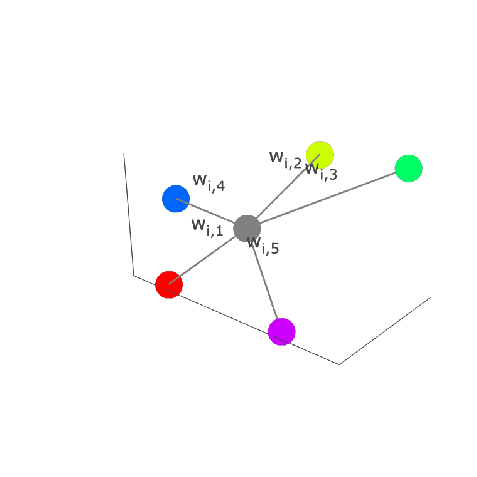
\includegraphics[trim = 50 50 20 60, clip, % left bottom right top
   width = 0.7\textwidth]{figures/reconstruction_3d}
 \end{subfigure}
 \hfill
 \begin{subfigure}[b]{0.48\textwidth}
   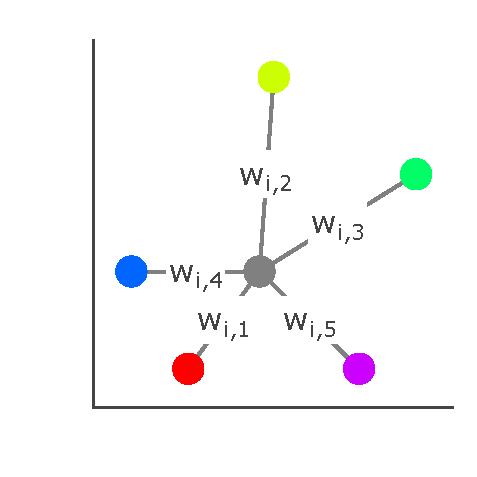
\includegraphics[trim = 40 30 0 20, clip, % left bottom right top
   width = 0.5\textwidth]{figures/reconstruction_2d}
 \end{subfigure}
\end{figure}

\end{frame}

% ------------------------------------------------------------------------------

\LARGE
\begin{frame}{\textcolor{gray!90}{3.1 unsupervised} ~~ lle}
\normalsize
\vspace{-0.5cm}
\noindent \textcolor{gray!90}{\rule{\textwidth}{1pt}}
\smallskip

\textbf{Reconstruction loss minimization:} finding optimal reconstruction 
weights

\begin{fleqn}
  \begin{equation}
    \small
    \min_{\W} \varepsilon(\W) = \min_{\W} \sum_i
    \twonorm{\x_i - \sum_j w_{ij} \x_j}, 
    \quad \text{s.t. } \bm{1}^T \bm{w}_i = 1 \quad \forall i \in \setN
  \end{equation}
\end{fleqn}

\textbf{Embedding loss minimization:} finding optimal embedding coordinates

\begin{fleqn}
  \begin{equation}
    \small
    \min_{\Y} \Phi(\Y) = \min_{\Y} \sum_i \twonorm{\y_i - \sum_j w_{ij} 
    \y_j},
    \quad  \text{s.t. } \frac{1}{N} \sum_i \y_i \y_i^T = \I,
    \quad \sum_i \y_i = \bm{0} \quad \forall i \in \setN
  \end{equation}
\end{fleqn}

\textbf{Eigenvalue problem:} define $\E = (\I - \W)^T(\I - \W)$ and set 
$\Ytil = \Y^T$, such that

\begin{fleqn}
  \begin{equation}
    \small
    \min_{\Ytil} \mathit{trace}(\Ytil^T \E \Ytil), \quad
    \text{s.t. } \frac{1}{N} \Ytil^T \Ytil = \I, \quad
    \Ytil^T\bm{1} = \bm{0}.
    \label{eq-lle-eigen}
  \end{equation}
\end{fleqn}

\conclbox{Solution: bottom $d + 1$ eigenvectors}

\end{frame}

% ------------------------------------------------------------------------------

\LARGE
\begin{frame}%<presentation:0>[noframenumbering]
{\textcolor{gray!90}{3.1 unsupervised} ~~ hlle}

\normalsize
\vspace{-0.5cm}
\noindent \textcolor{gray!90}{\rule{\textwidth}{1pt}}
\smallskip

\textbf{Proposal:} \citet{donohogrimes2003}

\vspace{0.3cm}

\textbf{Idea:} finding a truly linear mapping while preserving local 
isometry

\begin{itemize}
  \arritem Notion of curviness in mapping function
  \arritem Second-order penalty on Hessian
  \arritem Strong convergence guarantees but rather complex computations
\end{itemize}

\vspace{0.3cm}

\textbf{Solution:} eigenanalysis of empirical Hessian functional $\mathcal{H}$

\begin{itemize}
  \arritem Quadratic form of Hessian estimators in linear 
  neighborhood patches
  \arritem Discrete approximation of continuous Hesssian functional
  $\mathscr{H}(f)$
  \arritem Null space problem
\end{itemize}

% \textbf{Hessian functional}. Measuring average curviness over $\mani$
% 
% \begin{itemize}
%   \arritem Continuous functional. 
%   $\mathscr{H}(f) = \int_{\mani} \frobnorm{\Hes_f^{\text{loc}}(\pv)} d\pv$
%   \arritem Hessian estimators $\Hes_{\ell}$ derived from locally linear 
%   neighborhood patches
%   \arritem Empirical approximator.
%   $\mathcal{H}_{ij} = \sum_{\ell} \sum_m (\Hes_{\ell})_{m,i}
%   (\Hes_{\ell})_{m,j}$
%   \arritem Finding null space of $\mathcal{H}$
% \end{itemize}

\vfill

\conclbox{Solution: bottom $d + 1$ eigenvectors + scaling}

\end{frame}

% ------------------------------------------------------------------------------

\LARGE
\begin{frame}{\textcolor{gray!90}{3.2 semi-supervised} ~~ sslle}
\normalsize
\vspace{-0.5cm}
\noindent \textcolor{gray!90}{\rule{\textwidth}{1pt}}
\smallskip

\textbf{Proposal:} \citet{yangetal2006}

\vspace{0.3cm}

\textbf{Problem:} embedding found by unsupervised methods not always meaningful

\vspace{0.3cm}

\textbf{Idea:} improving LLE by use of prior knowledge

\vspace{0.3cm}

\textbf{Semi-supervision:} anchoring embedding at some prior points with known 
coordinates

\begin{itemize}
  \arritem More active than semi-supervised learning?
  \arritem Information available or to be obtained by querying the 
  oracle
  \arritem Maximum information at little expense $\Rightarrow$ careful 
  choice of prior points
\end{itemize}

% \vspace{0.3cm}

\begin{figure}[H]
 \begin{subfigure}[c]{0.2\textwidth}
  \centering
   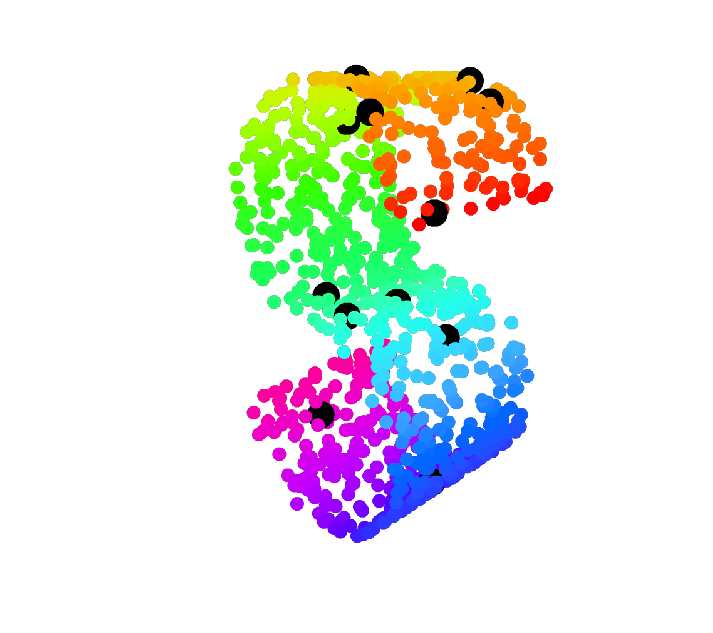
\includegraphics[trim = 70 30 70 30, clip, % left bottom right top
      width = 0.5\textwidth]{figures/s_curve_pp_random}
 \end{subfigure}
 \hfill
 \begin{subfigure}[c]{0.7\textwidth}
   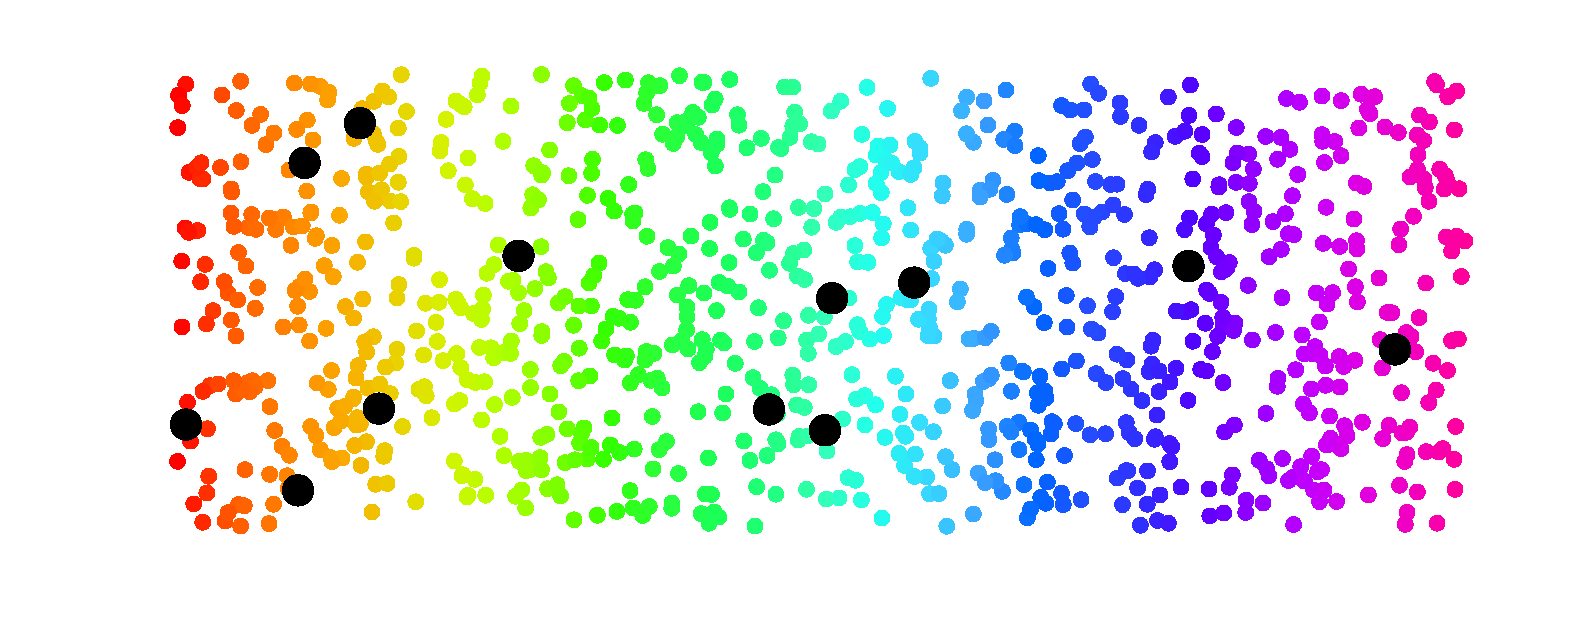
\includegraphics[trim = 80 20 0 0, clip, % left bottom right top
      width = 0.5\textwidth]{figures/s_curve_undone_pp_random}
 \end{subfigure}
\end{figure}

\end{frame}

% ------------------------------------------------------------------------------

\LARGE
\begin{frame}{\textcolor{gray!90}{3.2 semi-supervised} ~~ sslle}
\normalsize
\vspace{-0.5cm}
\noindent \textcolor{gray!90}{\rule{\textwidth}{1pt}}
\smallskip

% \textbf{Choice of prior points}. Basically, three options
% 
% \begin{itemize}
%   \arritem Pre-existing prior information
%   \arritem Random choice
%   \arritem Maximum exploration
% \end{itemize}
% 
% \vspace{0.3cm}

% \textbf{Types of prior information}. Exact vs inexact
% 
% \begin{itemize}
%   \arritem Level of confidence encoded in parameter
% \end{itemize}
% 
% \vspace{0.3cm}
% 
% \textbf{Algorithmic impact}. Recall LLE eigenvalue problem
% 
% \begin{fleqn}
%   \begin{equation*}
%     \small
%     \min_{\Y} \text{\textit{trace}}(\Y^T \E \Y), \quad
%     \text{s.t. } \frac{1}{N} \Y^T \Y = \I, \quad
%     \Y^T\bm{1} = \bm{0}.
%   \end{equation*}
% \end{fleqn}
% 
% $\Rightarrow$ Partitioning of $\E$ and $\Y$ 

% \begin{figure}[H]
%   \raggedright
%   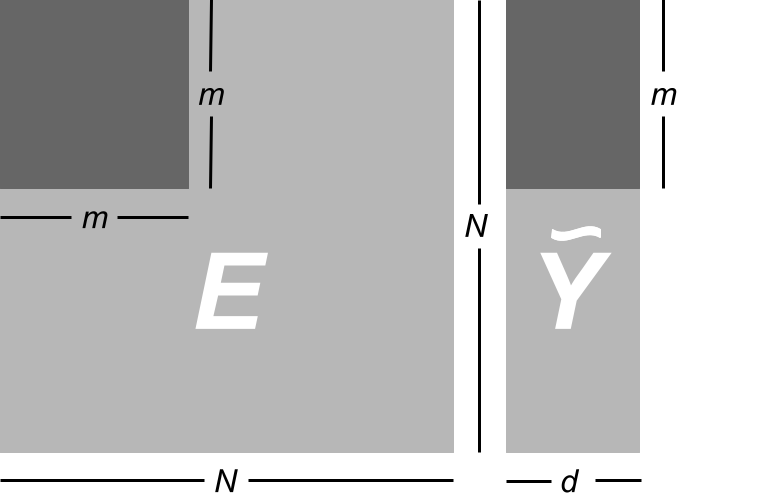
\includegraphics[trim = 0 0 0 0, clip, % left bottom right top
%   width = 0.4\textwidth]{figures/matrix_partition}
% \end{figure}

\textbf{Types of prior information:} exact vs inexact
\begin{itemize}
  \arritem Level of confidence encoded in parameter $\beta$
\end{itemize}
% \vspace{0.1cm}

\begin{minipage}[t]{0.6\textwidth}
\phantom{foo} \\
\textbf{Algorithmic impact:} recall LLE eigenvalue problem
\begin{fleqn}
  \begin{equation*}
    \min_{\Ytil} \mathit{trace}(\Ytil^T \E \Ytil), \quad
    \text{s.t. } \frac{1}{N} \Ytil^T \Ytil = \I, \quad
    \Ytil^T\bm{1} = \bm{0}.
  \end{equation*}
\end{fleqn}
$\Rightarrow$ partitioning of $\E$ and $\Ytil$ \\
\end{minipage}%
\begin{minipage}[t]{0.05\textwidth}
  \phantom{foo}
\end{minipage}%
\begin{minipage}[t]{0.35\textwidth}
  \begin{figure}[H]
    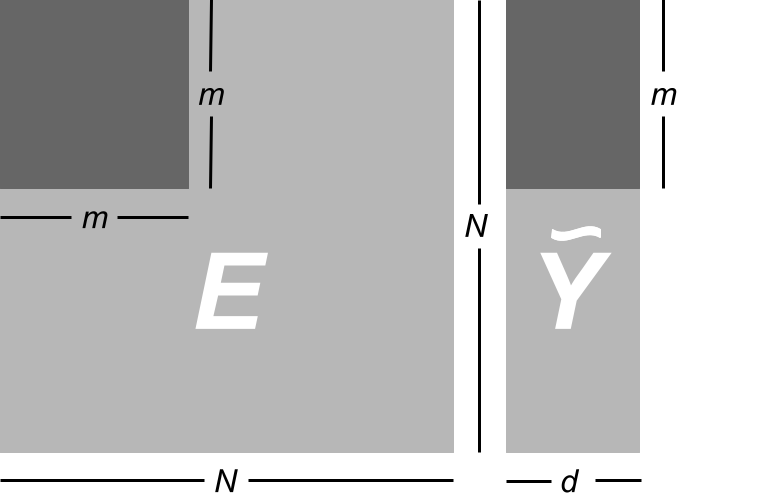
\includegraphics[trim = 0 0 0 0, clip, % left bottom right top
      width = 0.9\textwidth]{figures/matrix_partition}
  \end{figure}
\end{minipage}

\end{frame}

% ------------------------------------------------------------------------------

\LARGE
\begin{frame}{\textcolor{gray!90}{3.2 semi-supervised} ~~ sslle}
\normalsize
\vspace{-0.5cm}
\noindent \textcolor{gray!90}{\rule{\textwidth}{1pt}}
\smallskip

\textbf{Modified optimization problem:} exact information 

\begin{fleqn}
  \begin{equation}
    \min_{\Ytil_2}
    \begin{bmatrix} \textcolor{gray!90}{\Ytil_1} & \Ytil_2 \end{bmatrix}
    \begin{bmatrix} \textcolor{gray!90}{M_{11}} & M_{12} \\ M_{21} & M_{22} 
    \end{bmatrix}
    \begin{bmatrix} \textcolor{gray!90}{\Ytil_1^T} \\ \Ytil_2^T \end{bmatrix}
  \end{equation}
\end{fleqn}

\begin{fleqn}
  \begin{equation}
    \Leftrightarrow \Ytil_2^T = M_{22}^{-1} M_{12} 
    \textcolor{gray!90}{\Ytil_1^T}
  \end{equation}
\end{fleqn}

\textbf{Modified optimization problem:} inexact information 

\begin{fleqn}
  \begin{equation}
    \min_{\Ytil_1, \Ytil_2}
    \begin{bmatrix} \Ytil_1 & \Ytil_2 \end{bmatrix}
    \begin{bmatrix} M_{11} & M_{12} \\ M_{21} & M_{22} \end{bmatrix}
    \begin{bmatrix} \Ytil_1^T \\ \Ytil_2^T \end{bmatrix} +
    \beta \frobnorm{\Ytil_1^T - \textcolor{gray!90}{\hat{\Ytil}_1^T}}
  \end{equation}
\end{fleqn}

\begin{fleqn}
  \begin{equation}
    \Leftrightarrow \begin{bmatrix} \textcolor{gray!90}{M_{11}} +
    \beta \I & M_{12} \\ M_{21} & M_{22} \end{bmatrix}
    \begin{bmatrix} \Ytil_1^T \\ \Ytil_2^T \end{bmatrix} =
    \begin{bmatrix} \textcolor{gray!90}{\hat{\Ytil}_1^T} \\ \bm{0} 
    \end{bmatrix}
  \end{equation}
\end{fleqn}

\end{frame}

% ------------------------------------------------------------------------------

\LARGE
\begin{frame}{\textcolor{gray!90}{3.3 challenges} ~~ critical parameters}
\normalsize
\vspace{-0.5cm}
\noindent \textcolor{gray!90}{\rule{\textwidth}{1pt}}
\smallskip

\textbf{Choice of landmark points:} basically, three options

\begin{itemize}
  \flexitem{1} Pre-existing prior information $\Rightarrow$ worst case: poor 
  coverage
  \flexitem{2} (Uniform) random sampling
  \flexitem{3} Maximum coverage $\Rightarrow$ minimization of condition number 
  $\kappa(M_{22})$
\end{itemize}

% \begin{figure}[H]
%  \begin{subfigure}[c]{0.2\textwidth}
%   % \centering
%    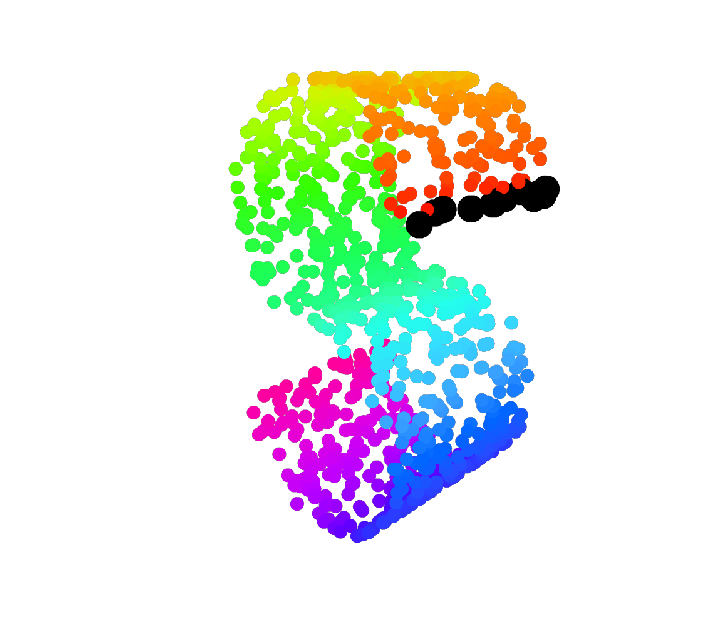
\includegraphics[trim = 80 20 60 0, clip, % left bottom right top
%       width = 0.8\textwidth]{figures/s-curve-pp-poor}
%  \end{subfigure}
%  \hfill
%  \begin{subfigure}[c]{0.2\textwidth}
%   % \centering
%    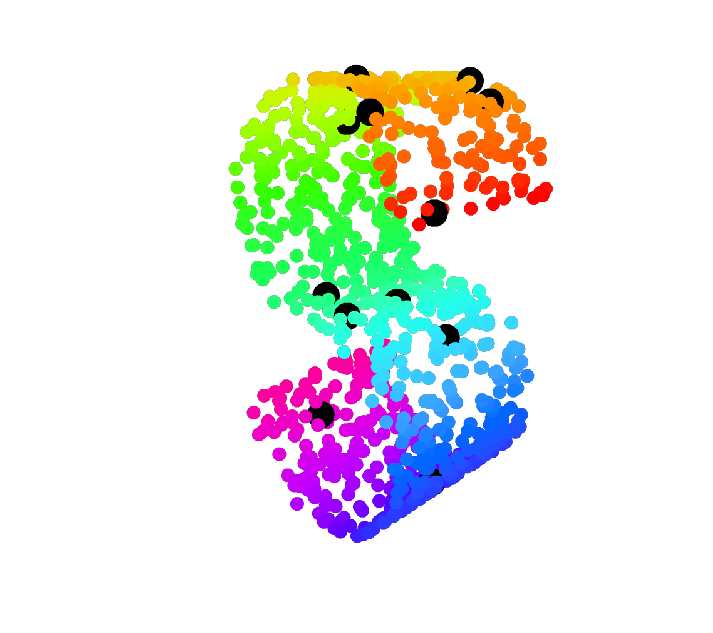
\includegraphics[trim = 80 20 60 0, clip, % left bottom right top
%       width = 0.8\textwidth]{figures/s-curve-pp-random}
%  \end{subfigure}
%  \hfill
%  \begin{subfigure}[c]{0.2\textwidth}
%    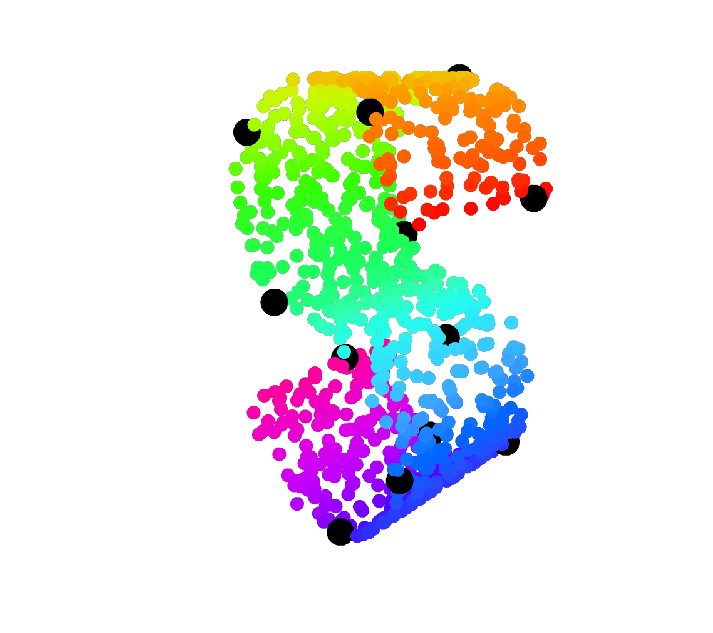
\includegraphics[trim = 80 20 60 0, clip, % left bottom right top
%       width = 0.8\textwidth]{figures/s-curve-pp-maxmin}
%  \end{subfigure}
% \end{figure}

\begin{minipage}[t]{0.33\textwidth}
  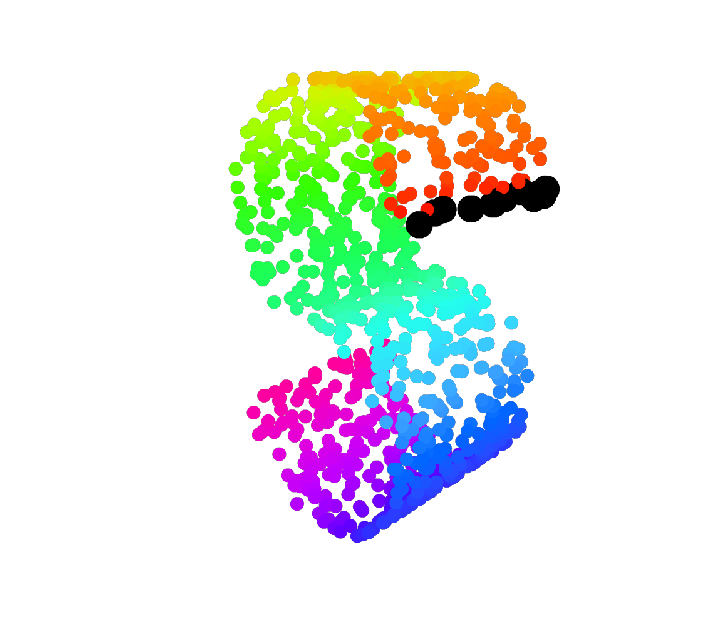
\includegraphics[trim = 80 20 60 0, clip, % left bottom right top
      width = 0.7\textwidth]{figures/s_curve_pp_poor}
\end{minipage}%
\begin{minipage}[t]{0.33\textwidth}
  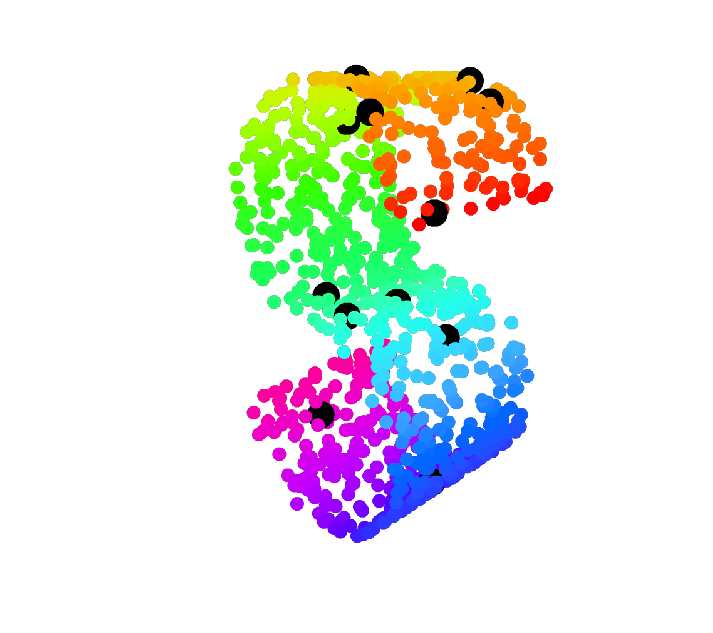
\includegraphics[trim = 80 20 60 0, clip, % left bottom right top
      width = 0.7\textwidth]{figures/s_curve_pp_random}
\end{minipage}%
\begin{minipage}[t]{0.33\textwidth}
    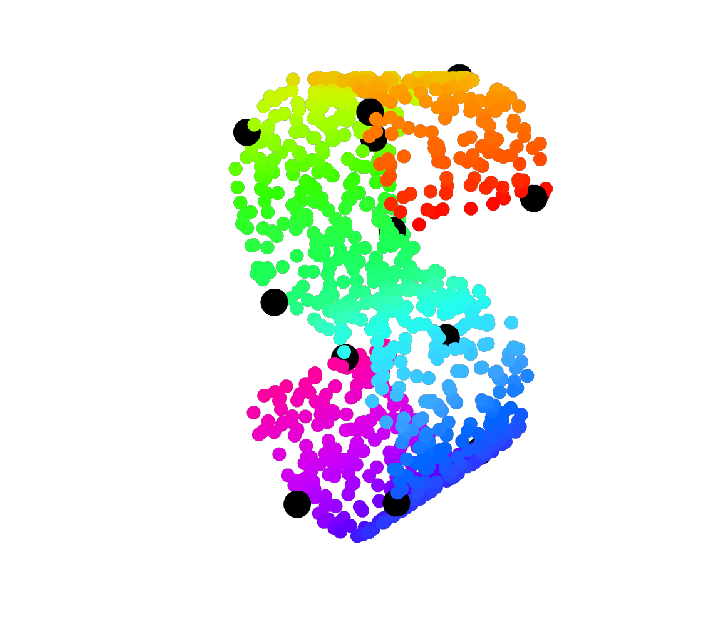
\includegraphics[trim = 80 20 60 0, clip, % left bottom right top
    width = 0.7\textwidth]{figures/s_curve_pp_maxmin}
\end{minipage}

% \vspace{0.3cm}
% 
% \textbf{Maximum coverage.} Points scattered across manifold surface
% 
% \begin{itemize}
%   \arritem Goodness of solution depending on condition number $\kappa(M_{22})$
%   \arritem $\kappa(M_{22})$ minimal at maximization of minimum pairwise 
%   distances between prior points
% \end{itemize}

\end{frame}

% ------------------------------------------------------------------------------

\LARGE
\begin{frame}{\textcolor{gray!90}{3.3 challenges} ~~ critical parameters}
\normalsize
\vspace{-0.5cm}
\noindent \textcolor{gray!90}{\rule{\textwidth}{1pt}}
\smallskip

% \vspace{0.3cm}

\textbf{Number \& location of prior points:} utility of prior knowledge ~ 
\maketag{analysis}

\begin{itemize}
  \arritem Exploration vs labeling cost
\end{itemize}

\textbf{Noise level:} quality of prior knowledge ~ 
\maketag{analysis}

\begin{itemize}
  \arritem Support vs harm through prior knowledge
\end{itemize}

\textbf{Confidence parameter:} strength of belief in prior knowledge 
% ~ \maketag{analysis}

\begin{itemize}
  \arritem Rather robust
\end{itemize}

% \textbf{Intrinsic dimensionality}. True sources of variability
% 
% \begin{itemize}
%   \arritem Considered known with availability of prior information
% \end{itemize}

\vspace{0.3cm}

\textbf{Further hyperparameters:} also critical in unsupervised case

\begin{itemize}
  \flexitem{1} Intrinsic dimensionality
  \flexitem{2} Neighborhood size
  \flexitem{3} Regularization constant
\end{itemize}
% 
% \textbf{Neighborhood size}. Global vs local structure
% 
% \begin{itemize}
%   \arritem Tunable (expensive)
% \end{itemize}
% 
% % \vspace{0.3cm}
% 
% \textbf{Regularization constant}. Singularity for $D < k$
% 
% \begin{itemize}
%   \arritem Heuristics
% \end{itemize}


\end{frame}

% ------------------------------------------------------------------------------
% SENSITIVITY ANALYSIS
% ------------------------------------------------------------------------------

\LARGE
\begin{frame}[noframenumbering]{\phantom{foo}}
\normalsize
\vspace{-0.5cm}
\noindent \textcolor{gray!90}{\rule{\textwidth}{1pt}}
\smallskip

\Huge
\hspace{0pt}
\vfill
\textbf{\highlight{~~ 4 ~~ SENSITIVITY ANALYSIS}}
\vfill
\hspace{0pt}

\noindent \textcolor{gray!90}{\rule{\textwidth}{1pt}}

\end{frame}

% ------------------------------------------------------------------------------

\LARGE
\begin{frame}{\textcolor{gray!90}{4.1 setup} ~~ data}
\normalsize
\vspace{-0.5cm}
\noindent \textcolor{gray!90}{\rule{\textwidth}{1pt}}
\smallskip

\textbf{Data:} two data sets, $N = 1000$ observations each

\begin{minipage}[b]{0.65\textwidth}
  \textbf{Swiss roll:} \textit{the} standard synthetic manifold
  \begin{itemize}
    \flexitem{1} Sample $\bm{u}_1, \bm{u}_2 \sim U(0, 1)$ 
    $\mathit{ iid}$ with $\rvert \bm{u}_1 \rvert = \rvert \bm{u}_1 \rvert = N$
    \flexitem{2} Compute $\bm{t} = 1.5 \pi (1 + 2\bm{u}_1)$ and 
    $\bm{s} = 21 \bm{u}_2$
    \flexitem{3} $\X_{\text{swiss}} = 
    \begin{bmatrix} \x_1 & \x_2 & \x_3 \end{bmatrix} =
    \begin{bmatrix} \bm{t} \cos{\bm{t}} & \bm{s} & 
    \bm{t} \sin{\bm{t}} \end{bmatrix}$ 
  \end{itemize}
\end{minipage}%
\begin{minipage}[b]{0.35\textwidth}
  \centering
  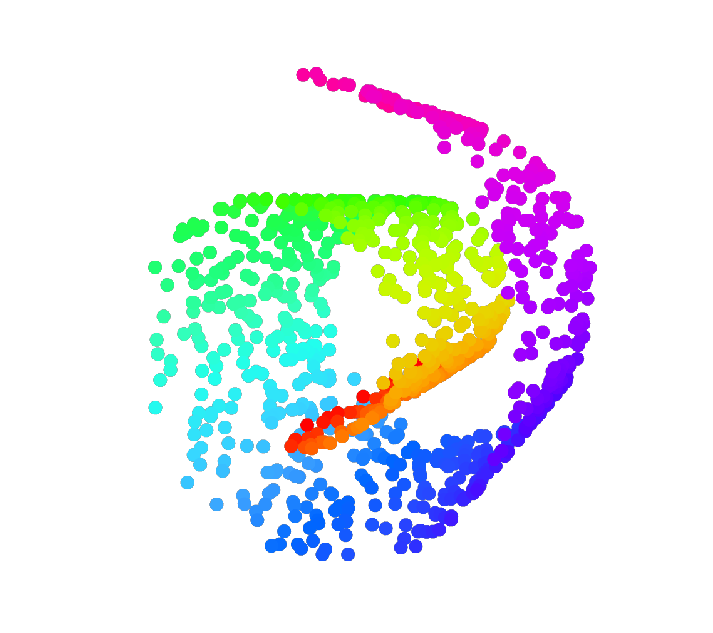
\includegraphics[trim = 60 30 40 -20, clip, % left bottom right top
    width = 0.45\textwidth]{figures/swiss_roll}
\end{minipage}

\vspace{0.3cm}

\begin{minipage}[b]{0.65\textwidth}
  \textbf{Incomplete tire:} examined in \citet{yangetal2006}
  \begin{itemize}
    \flexitem{1} Sample $\bm{u}_1, \bm{u}_2 \sim U(0, 1)$ 
    $\mathit{ iid}$ with $\rvert \bm{u}_1 \rvert = \rvert \bm{u}_1 \rvert = N$
    \flexitem{2} Compute $\bm{t} = \frac{5 \pi}{3} \bm{u}_1$ and 
    $\bm{s} = \frac{5 \pi}{3} \bm{u}_2$
    \flexitem{3} 
    $\X_{\text{tire}} =
    \begin{bmatrix} \x_1 & \x_2 & \x_3 \end{bmatrix} $ \\
    \phantom{$\X_{\text{tire}}$} $ = \begin{bmatrix} (3 + \cos{\bm{s}}) 
    \cos{\bm{t}} & (3 + \cos{\bm{s}}) \sin{\bm{t}} & \sin{\bm{s}} \end{bmatrix}$
  \end{itemize}
\end{minipage}%
\begin{minipage}[b]{0.35\textwidth}
  \centering
  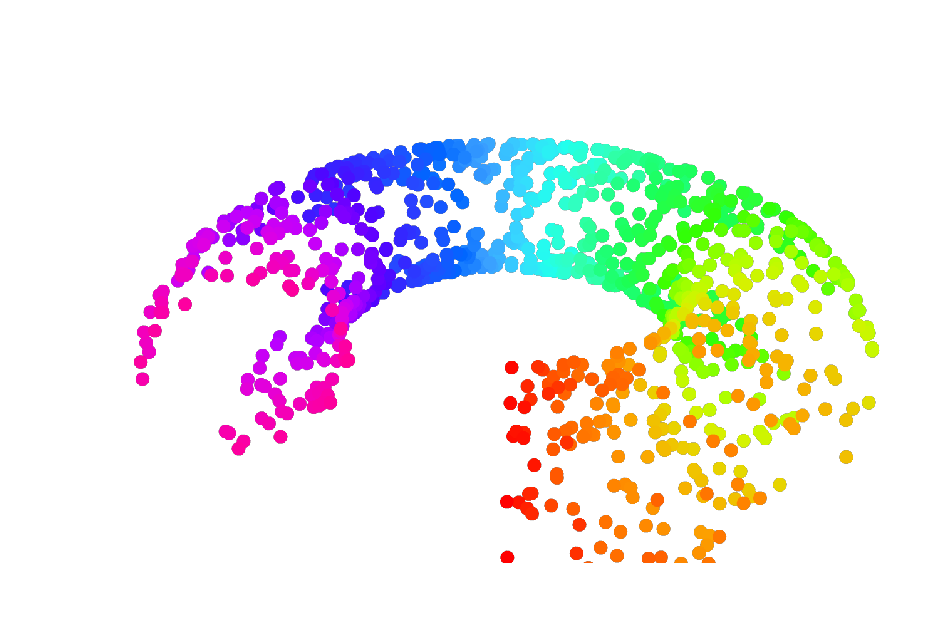
\includegraphics[trim = 20 0 0 0, clip, % left bottom right top
    width = 0.7\textwidth]{figures/incomplete_tire}
\end{minipage}

\end{frame}

% ------------------------------------------------------------------------------

\LARGE
\begin{frame}{\textcolor{gray!90}{4.1 setup} ~~ scenarios}
\normalsize
\vspace{-0.5cm}
\noindent \textcolor{gray!90}{\rule{\textwidth}{1pt}}
\smallskip

\conclbox{Sensitivity analysis \phantom{I}I: ~~ landmark coverage $\times$ 
number of landmark points} 

\vspace{0.3cm}

\begin{itemize}
  \arritem Landmark coverage $\in \{ \text{poor}, \text{ random}, 
  \text{ maximum}\}$
  \arritem Number of landmark points $\in \{2, 4, 6, 8, 10, 12\}$
\end{itemize}

% \vspace{0.3cm}
% 
% $\Rightarrow$ Best case: maximum coverage \& 12 landmarks

\vfill

\conclbox{Sensitivity analysis II: ~~ noise level $\times$ number of landmark 
points}

\vspace{0.3cm}

\begin{itemize}
  \arritem Landmark coverage kept at optimal configuration
  \arritem Simulation of inexact prior information through additive Gaussian 
  noise 
  \arritem Corruption of landmark $\pv$ as 
  $\tilde{\pv} = \pv + \bm{\epsilon} = (p_t, p_s) + (\epsilon_t, \epsilon_s)$ \\
  with $\epsilon_i \sim N(0, (\alpha \cdot s_i)^2) ~ \mathit{iid}$,
  scaled by empirical variance $s_i$, $i \in \{t, s\}$
  % $(\epsilon_t, \epsilon_s) \sim N(\bm{0}, 
  % \mathit{diag}(\sigma_t^2, \sigma_s^2))$
  % \arritem Perturbation scaled by empirical variance $s_i$ 
  % $\Rightarrow$ $\sigma_i = \alpha \cdot s_i$
  \arritem Noise level $\alpha \in \{0.1, 0.5, 1.0, 3.0\}$ 
  \arritem Number of landmark points $\in \{2, 4, 6, 8, 10, 12\}$
\end{itemize}

% \vspace{0.3cm}
% 
% $\Rightarrow$ Best case: noise level 0.1 \& 12 landmarks

\end{frame}

% ------------------------------------------------------------------------------

\LARGE
\begin{frame}{\textcolor{gray!90}{4.1 setup} ~~ evaluation}
\normalsize
\vspace{-0.5cm}
\noindent \textcolor{gray!90}{\rule{\textwidth}{1pt}}
\smallskip

\textbf{Evaluation criterion:} $\text{AUC}(R_{NX})$ 
(\citet{kraemeretal2019}, \citet{lueksetal2011})

\begin{itemize}
  \arritem Area under the $R_{NX}$ curve
  \arritem Based on co-ranking matrix
\end{itemize}

\vspace{0.3cm}

\textbf{Co-ranking matrix:} comparing distance ranks in observation \& embedding 
spaces

\begin{itemize}
  \arritem Rank distance matrices $(r)_{ij}^{\text{obs}}, (r)_{ij}^{\text{emb}} 
  \in \R^{N \times N}$
  \arritem Co-ranking matrix $\bm{Q} = (q)_{\ell m} \in \R^{N \times N}$ with 
  $q_{\ell m} = 
  \big \rvert \{ (i, j): 
  r_{ij}^{\text{emb}} = \ell \land r_{ij}^{\text{obs}} = m \} \big \rvert$ 
  \arritem Interpretation:
  \begin{itemize}
    \flexitem{1} All non-zero entries on diagonal $\Rightarrow$ optimal 
    embedding
    \flexitem{2} Most non-zero entries on upper triangle $\Rightarrow$ close 
    points torn apart
    \flexitem{3} Most non-zero entries on lower triangle $\Rightarrow$ faraway 
    points collapsed
  \end{itemize}
\end{itemize}

\end{frame}

% ------------------------------------------------------------------------------

\LARGE
\begin{frame}{\textcolor{gray!90}{4.1 setup} ~~ evaluation}
\normalsize
\vspace{-0.5cm}
\noindent \textcolor{gray!90}{\rule{\textwidth}{1pt}}
\smallskip

\textbf{Co-ranking-based metrics:}

\begin{itemize}
  \arritem Number of points remaining in $k$-neighborhood after projection: 
  $Q_{NX}(k) = \dfrac{1}{kN} \sum_{\ell = 1}^k \sum_{m = 1}^k 
  q_{\ell m}$
  \arritem 
  % Adjustment for random embeddings and normalization. \\ 
  $R_{NX}(k) = \dfrac{(N - 1) Q_{NX}(k) - k}{N - 1 - k}$
\end{itemize}

\vspace{0.3cm}

\begin{minipage}[b]{0.6\textwidth}
  \textbf{AUC measure:} % Parameter-free
  \begin{itemize}
    \arritem $\text{AUC}(R_{NX}) = \dfrac{\sum_{k = 1}^{N - 2} R_{NX}(k)}{
    \sum_{k = 1}^{N - 2} 1 / k} \in [0, 1]$
    \arritem Interpretation:
    \begin{itemize}
      \flexitem{1} $\text{AUC}(R_{NX}) = 0$ $\Rightarrow$ random embedding
      \flexitem{2} $\text{AUC}(R_{NX}) = 1$ $\Rightarrow$ optimal embedding
    \end{itemize}
\end{itemize}
\end{minipage}%
\begin{minipage}[b]{0.4\textwidth}
  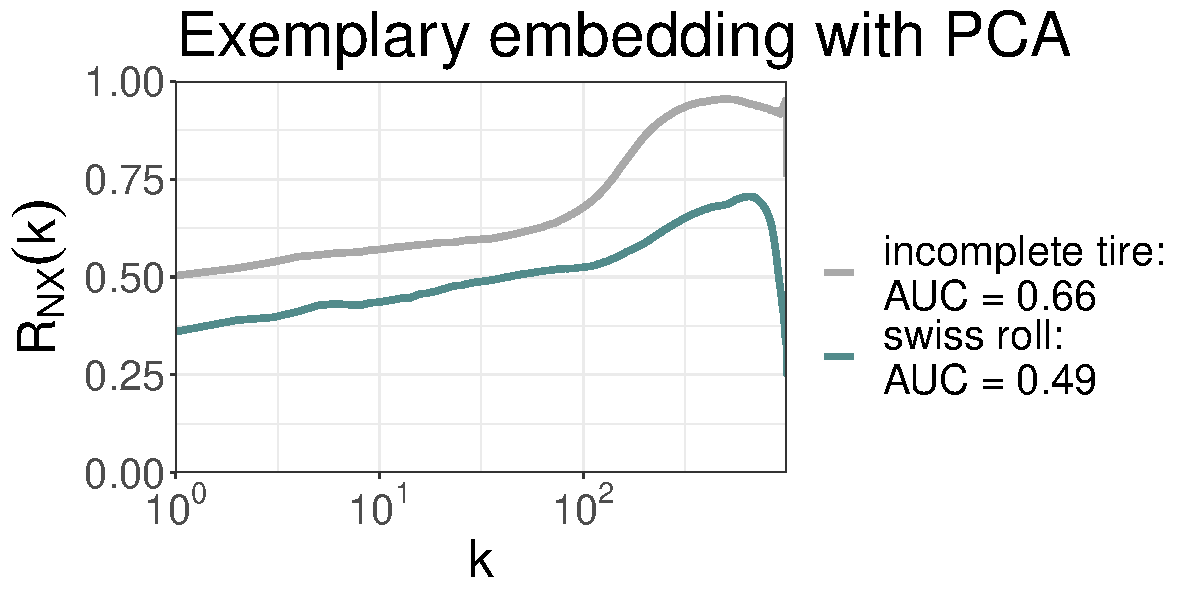
\includegraphics[trim = 0 0 0 0, clip, % left bottom right top
    width = \textwidth]{figures/rnx_curve}
\end{minipage}

\end{frame}

% ------------------------------------------------------------------------------

\LARGE
\begin{frame}{\textcolor{gray!90}{4.2 results} ~~ sensitivity analysis I}
\normalsize
\vspace{-0.5cm}
\noindent \textcolor{gray!90}{\rule{\textwidth}{1pt}}
\smallskip

\textbf{Key variation:} poor, random, maximum coverage

\vspace{0.3cm}

\begin{minipage}[c]{0.2\textwidth}
  Swiss roll
\end{minipage}%
\begin{minipage}[c]{0.8\textwidth}
  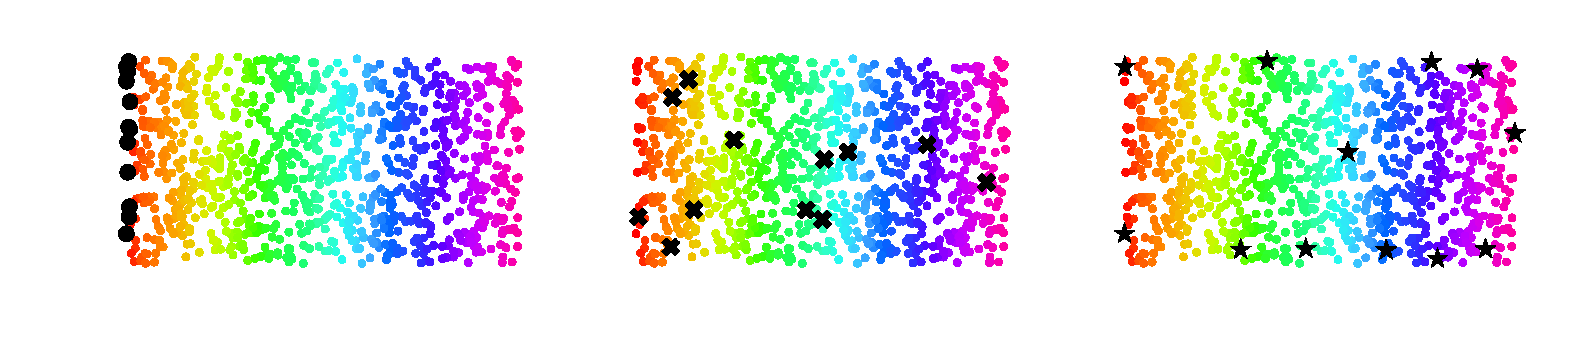
\includegraphics[trim = 40 20 0 0, clip, % left bottom right top
    width = \textwidth]{figures/sensitivity_landmarks_key_swiss_roll}
\end{minipage}

\vspace{0.3cm}   

\begin{minipage}[c]{0.2\textwidth}
  Incomplete tire
\end{minipage}%
\begin{minipage}[c]{0.8\textwidth}
  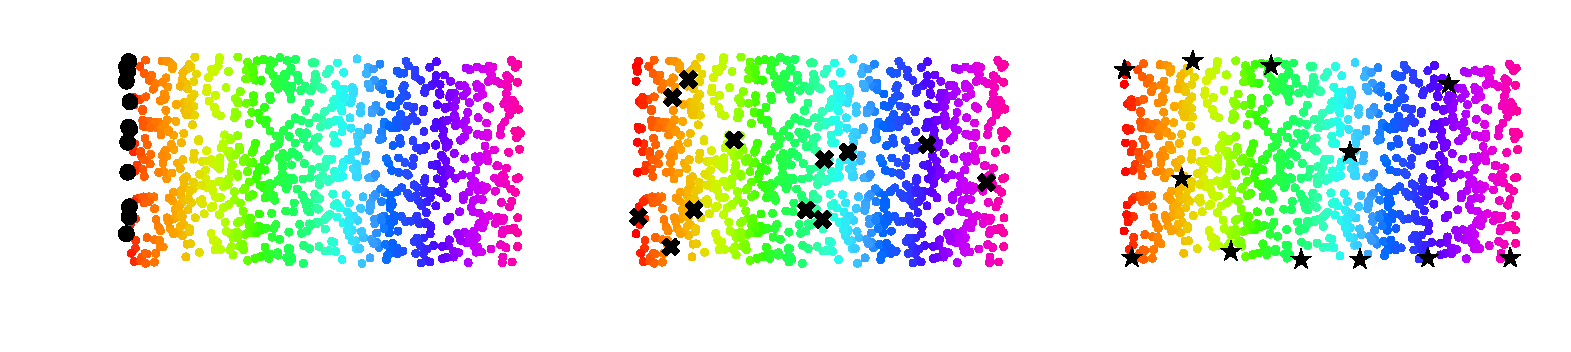
\includegraphics[trim = 40 20 0 0, clip, % left bottom right top
    width = \textwidth]{figures/sensitivity_landmarks_key_incomplete_tire}
\end{minipage}

\vfill

\scriptsize
$\bullet$ ~ poor coverage ~~~ $\bm{\times}$ ~ random coverage ~~~
$\star$ ~ maximum coverage

\end{frame}

% ------------------------------------------------------------------------------

\LARGE
\begin{frame}{\textcolor{gray!90}{4.2 results} ~~ sensitivity analysis I}
\normalsize
\vspace{-0.5cm}
\noindent \textcolor{gray!90}{\rule{\textwidth}{1pt}}
\smallskip

\textbf{Quantitative results:} seemingly better performance of random coverage

\vspace{0.3cm}

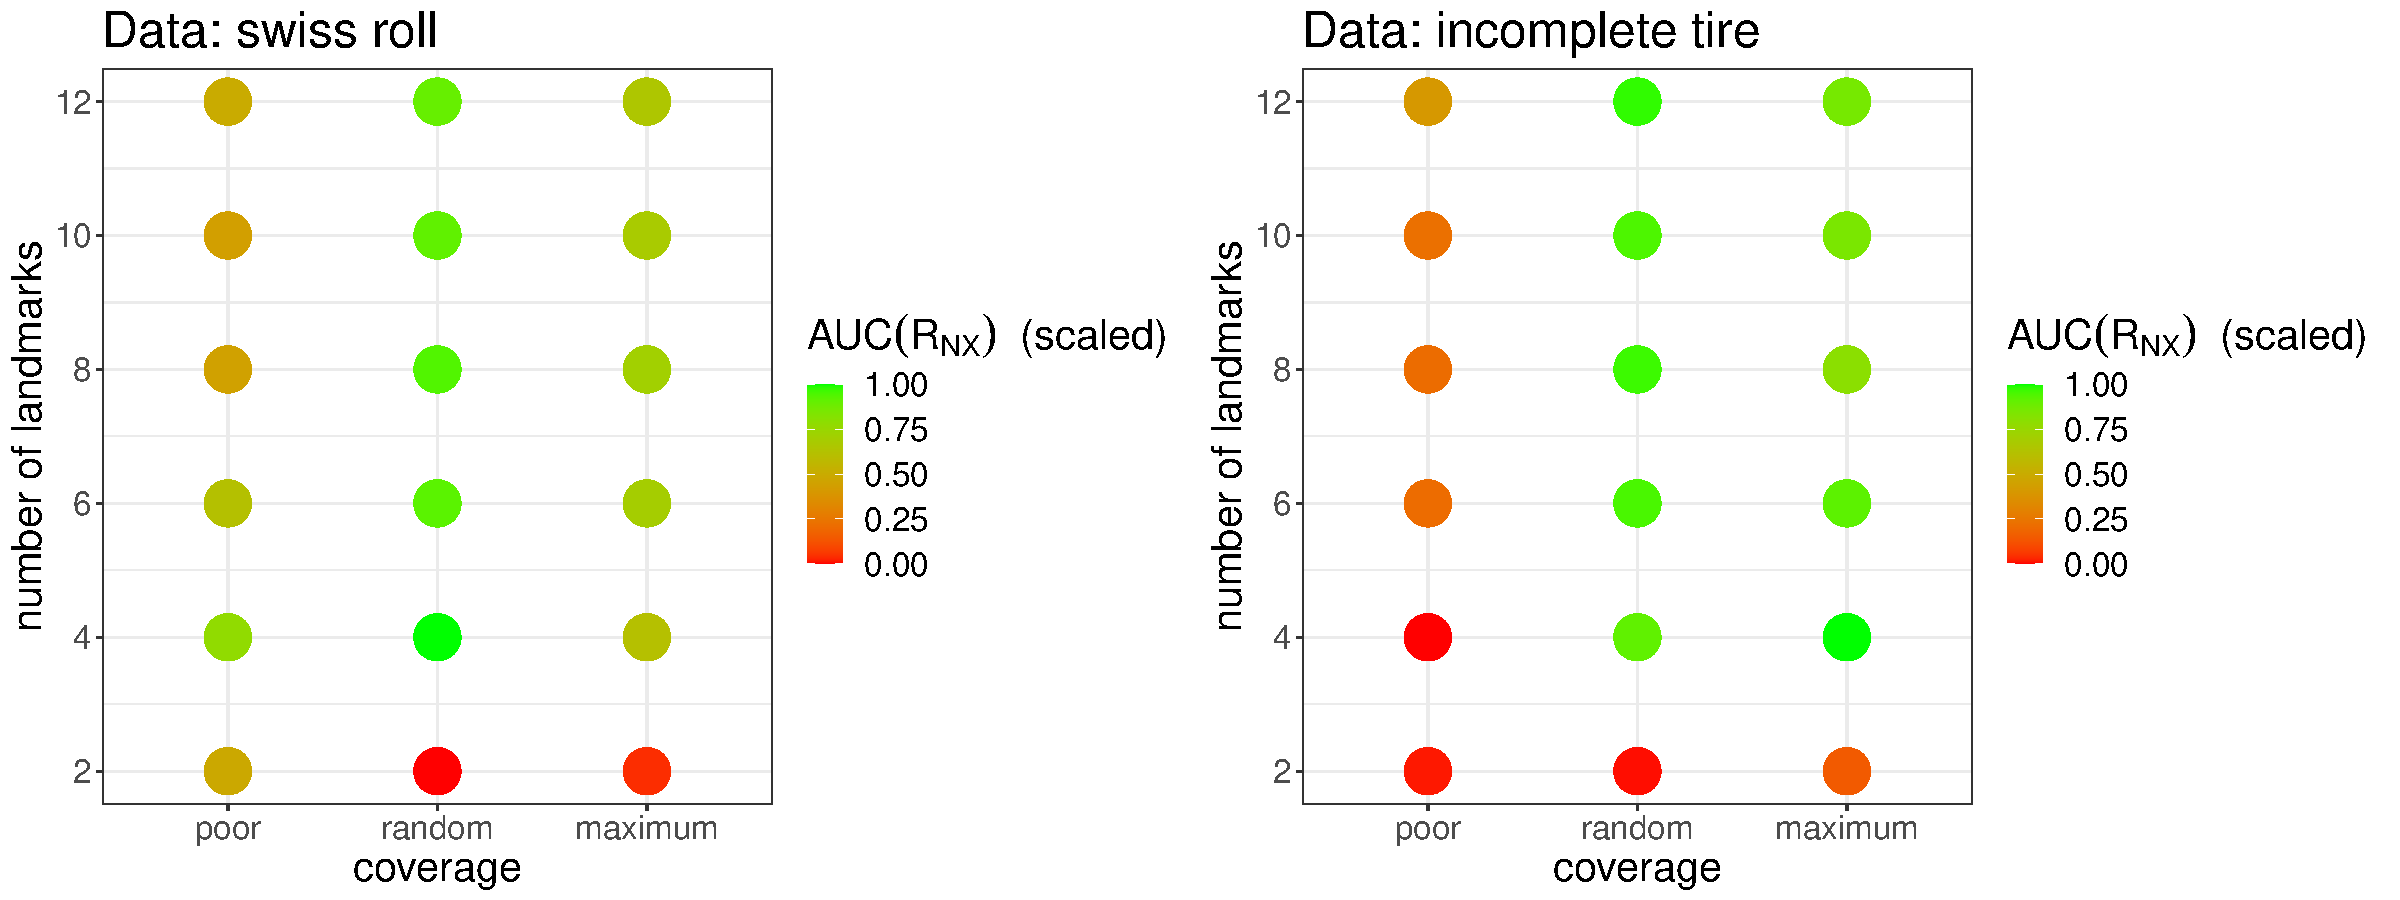
\includegraphics[trim = 0 0 0 0, clip, % left bottom right top
    width = \textwidth]{figures/sensitivity_landmarks_auc}
    
\vfill

\scriptsize
$\text{AUC}(R_{NX})$ has been scaled to take on a minimum of 0 and maximum of 1 
in both figures for better visibility of differences. \\
Original scales: swiss roll -- $\text{AUC}(R_{NX}) \in [0.2655, 0.4086]$, 
incomplete tire -- $\text{AUC}(R_{NX}) \in [0.2772, 0.6231]$

\end{frame}

% ------------------------------------------------------------------------------

\LARGE
\begin{frame}{\textcolor{gray!90}{4.2 results} ~~ sensitivity analysis I}
\normalsize
\vspace{-0.5cm}
\noindent \textcolor{gray!90}{\rule{\textwidth}{1pt}}
\smallskip

\textbf{Qualitative results:} swiss roll

\vspace{0.3cm}

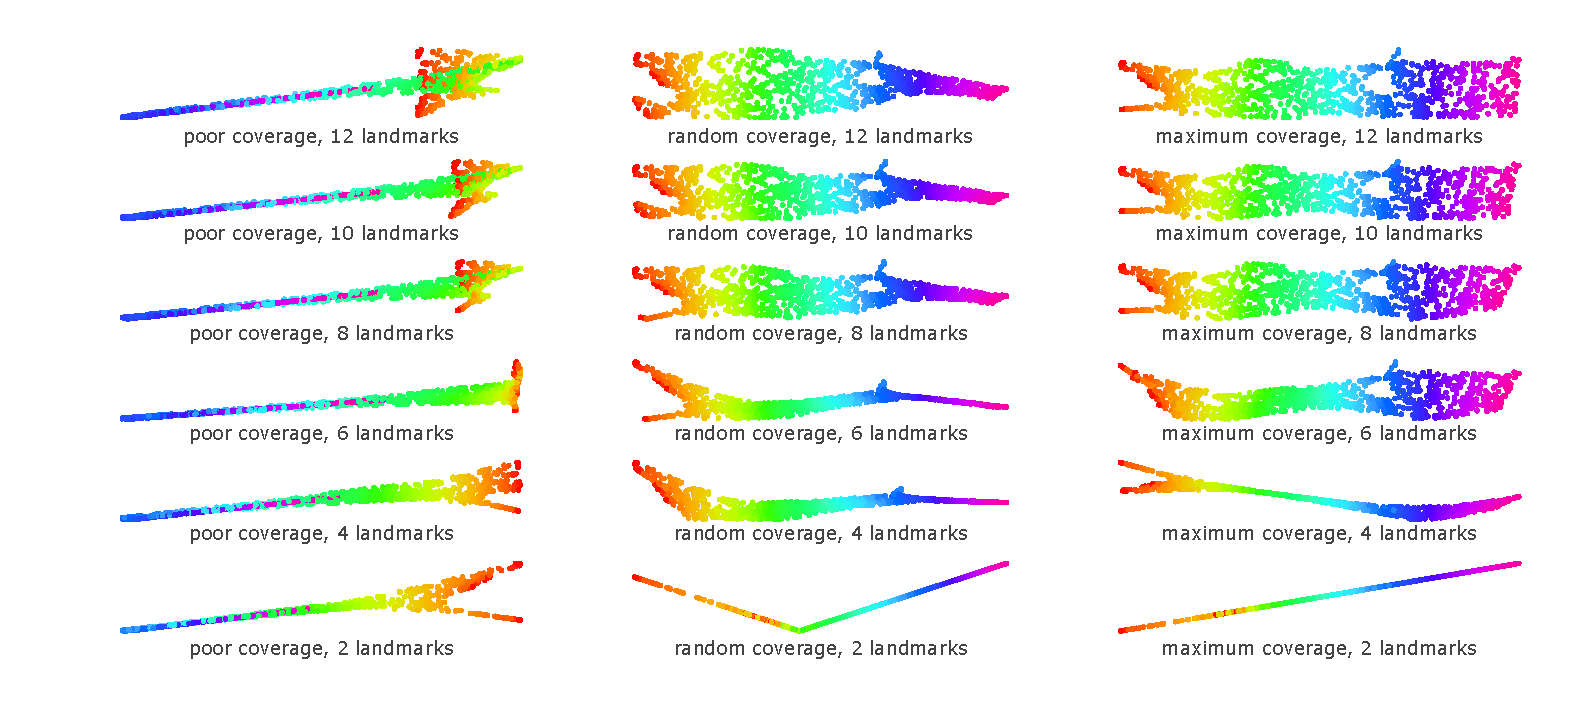
\includegraphics[trim = 40 10 0 0, clip, % left bottom right top
    width = \textwidth]{figures/sensitivity_landmarks_qual_swiss_roll}

\end{frame}

% ------------------------------------------------------------------------------

\LARGE
\begin{frame}{\textcolor{gray!90}{4.2 results} ~~ sensitivity analysis I}
\normalsize
\vspace{-0.5cm}
\noindent \textcolor{gray!90}{\rule{\textwidth}{1pt}}
\smallskip

\textbf{Qualitative results:} incomplete tire

\vspace{0.3cm}

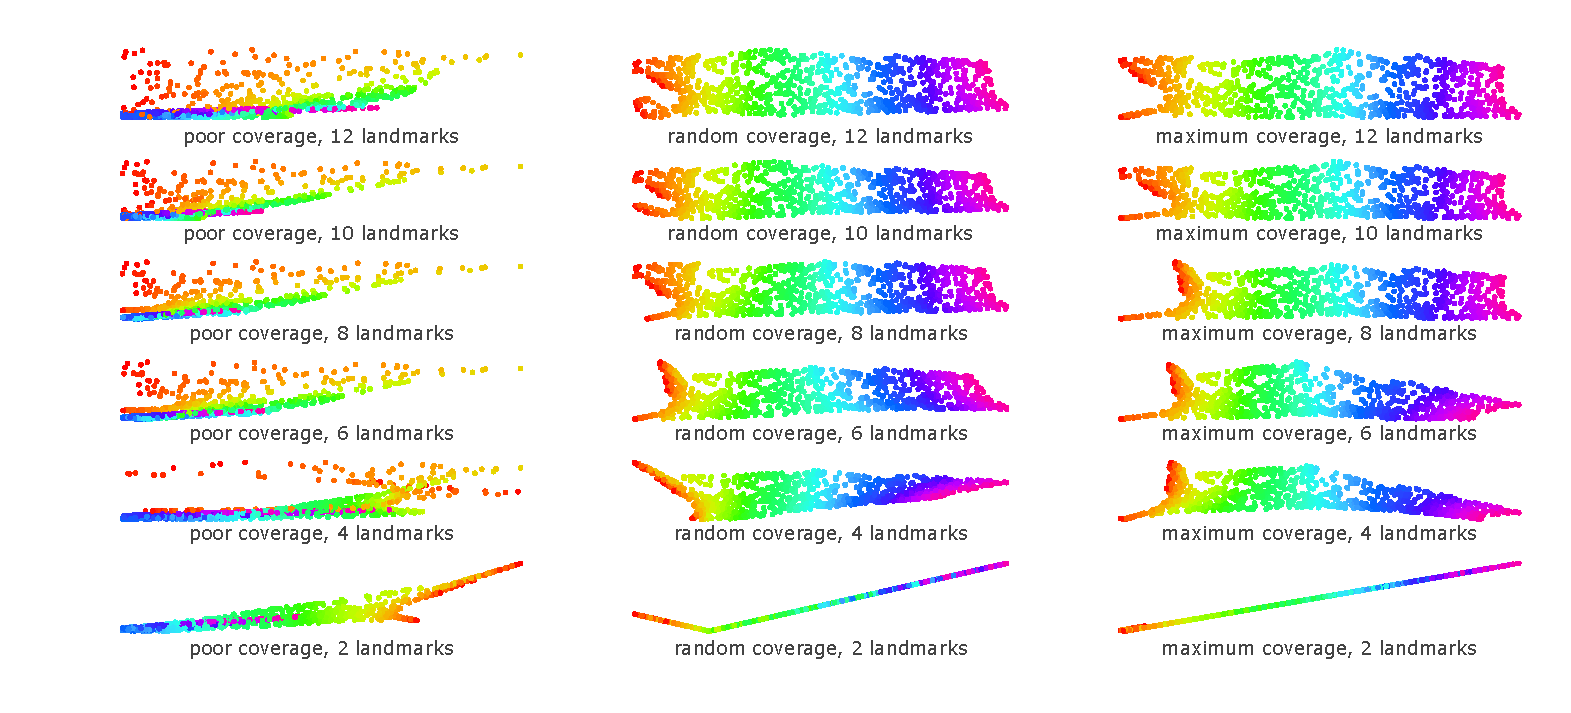
\includegraphics[trim = 40 10 0 0, clip, % left bottom right top
    width = \textwidth]{figures/sensitivity_landmarks_qual_incomplete_tire}

\end{frame}

% ------------------------------------------------------------------------------

\LARGE
\begin{frame}{\textcolor{gray!90}{4.2 results} ~~ sensitivity analysis II}
\normalsize
\vspace{-0.5cm}
\noindent \textcolor{gray!90}{\rule{\textwidth}{1pt}}
\smallskip

\textbf{Key variation:} noise level $\alpha \in \{0.1, 0.5, 1.0, 3.0\}$ 

\vspace{0.3cm}

\begin{minipage}[c]{0.2\textwidth}
  Swiss roll
\end{minipage}%
\begin{minipage}[c]{0.8\textwidth}
  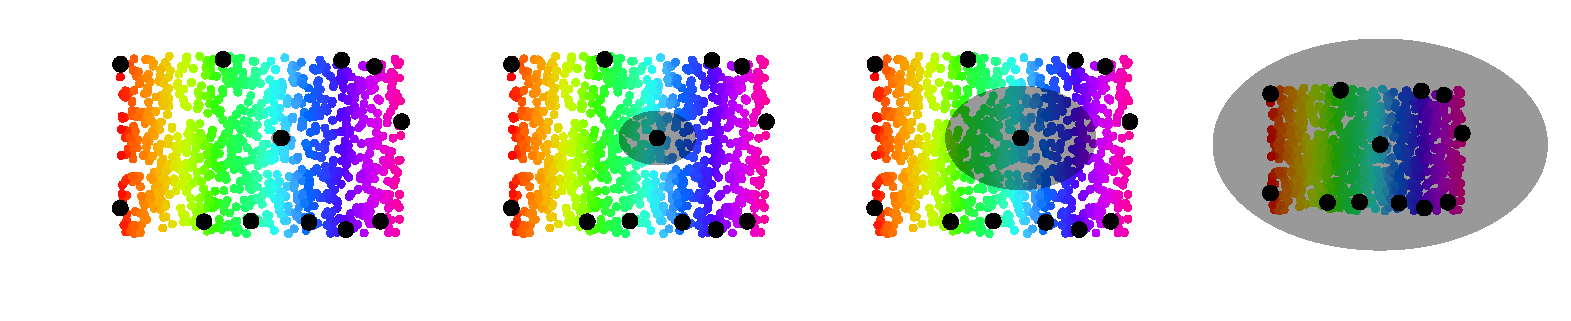
\includegraphics[trim = 40 30 0 0, clip, % left bottom right top
    width = \textwidth]{figures/sensitivity_noise_key_swiss_roll}
\end{minipage}

\vspace{0.3cm}   

\begin{minipage}[c]{0.2\textwidth}
  Incomplete tire
\end{minipage}%
\begin{minipage}[c]{0.8\textwidth}
  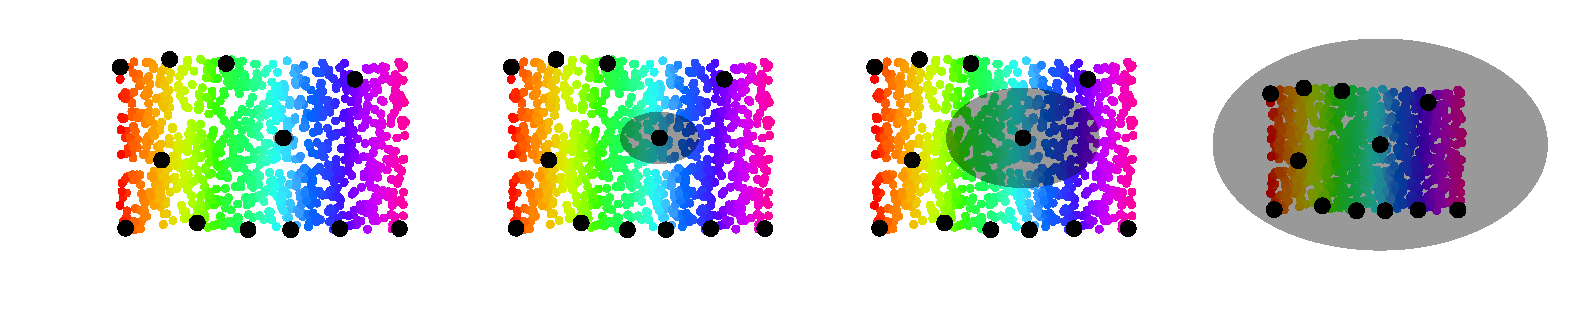
\includegraphics[trim = 40 30 0 0, clip, % left bottom right top
    width = \textwidth]{figures/sensitivity_noise_key_incomplete_tire}
\end{minipage}

\vfill

\scriptsize
Potential displacement by random noise, exemplified at one prior point location. 
\\
Ellipses have semi-axes of length = one standard deviation of the Gaussian noise 
variable, i.e., noise level scaled by standard deviation $s_i$ in $t$ and $s$ 
direction, respectively: $\alpha \cdot s_i$ with $i \in \{t, s\}$. \\
Landmarks have been found via maximum coverage.

\end{frame}

% ------------------------------------------------------------------------------

\LARGE
\begin{frame}{\textcolor{gray!90}{4.2 results} ~~ sensitivity analysis II}
\normalsize
\vspace{-0.5cm}
\noindent \textcolor{gray!90}{\rule{\textwidth}{1pt}}
\smallskip

\textbf{Quantitative results:} some compensation of noise by larger number of 
landmarks

\vspace{0.3cm}

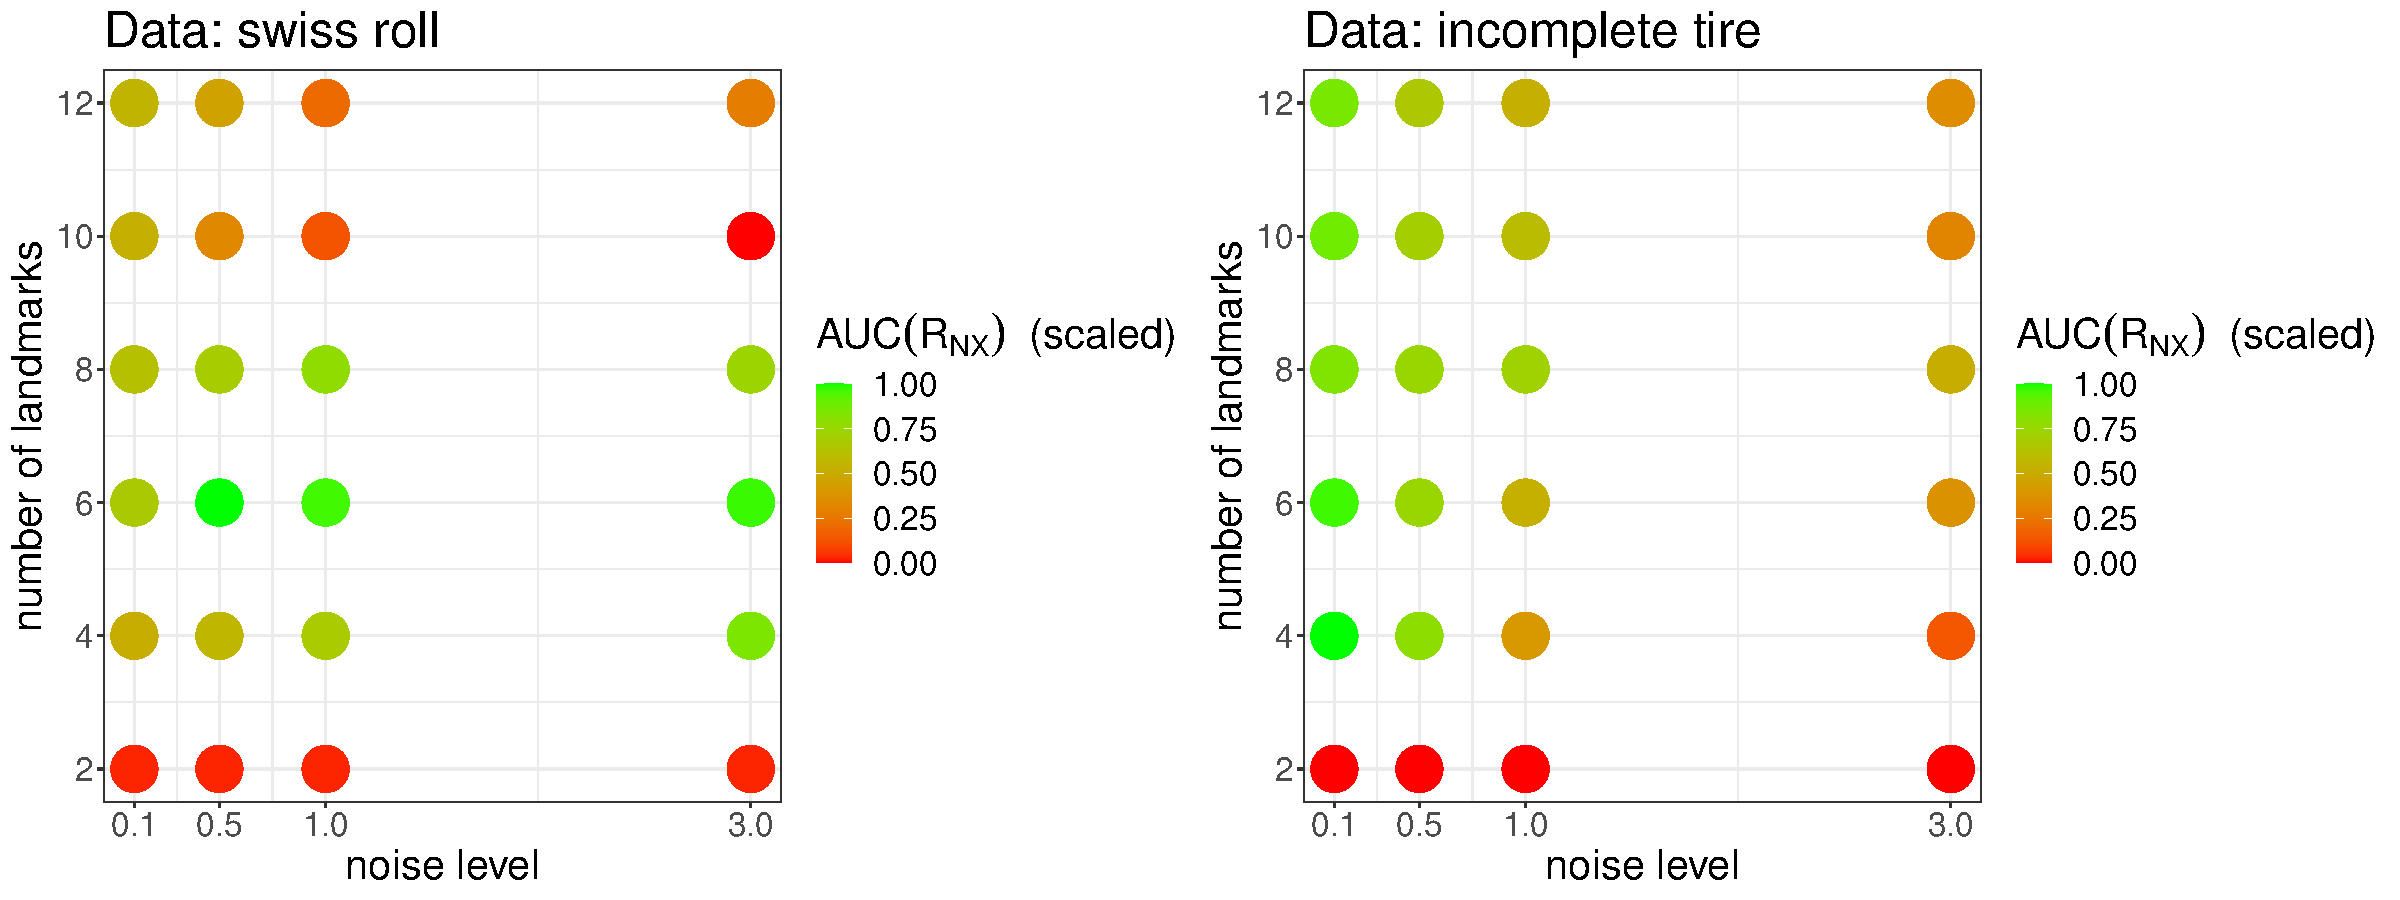
\includegraphics[trim = 0 0 0 0, clip, % left bottom right top
    width = \textwidth]{figures/sensitivity_noise_auc}

\vspace{0.3cm}

\scriptsize
$\text{AUC}(R_{NX})$ has been scaled to take on a minimum of 0 and maximum of 1 
in both figures for better visibility of differences. \\
Original scales: swiss roll -- $\text{AUC}(R_{NX}) \in [0.2720, 0.4167]$, 
incomplete tire -- $\text{AUC}(R_{NX}) \in [0.3171, 0.6172]$

\end{frame}

% ------------------------------------------------------------------------------

\LARGE
\begin{frame}{\textcolor{gray!90}{4.2 results} ~~ sensitivity analysis II}
\normalsize
\vspace{-0.5cm}
\noindent \textcolor{gray!90}{\rule{\textwidth}{1pt}}
\smallskip

\textbf{Qualitative results:} swiss roll

\vspace{0.3cm}

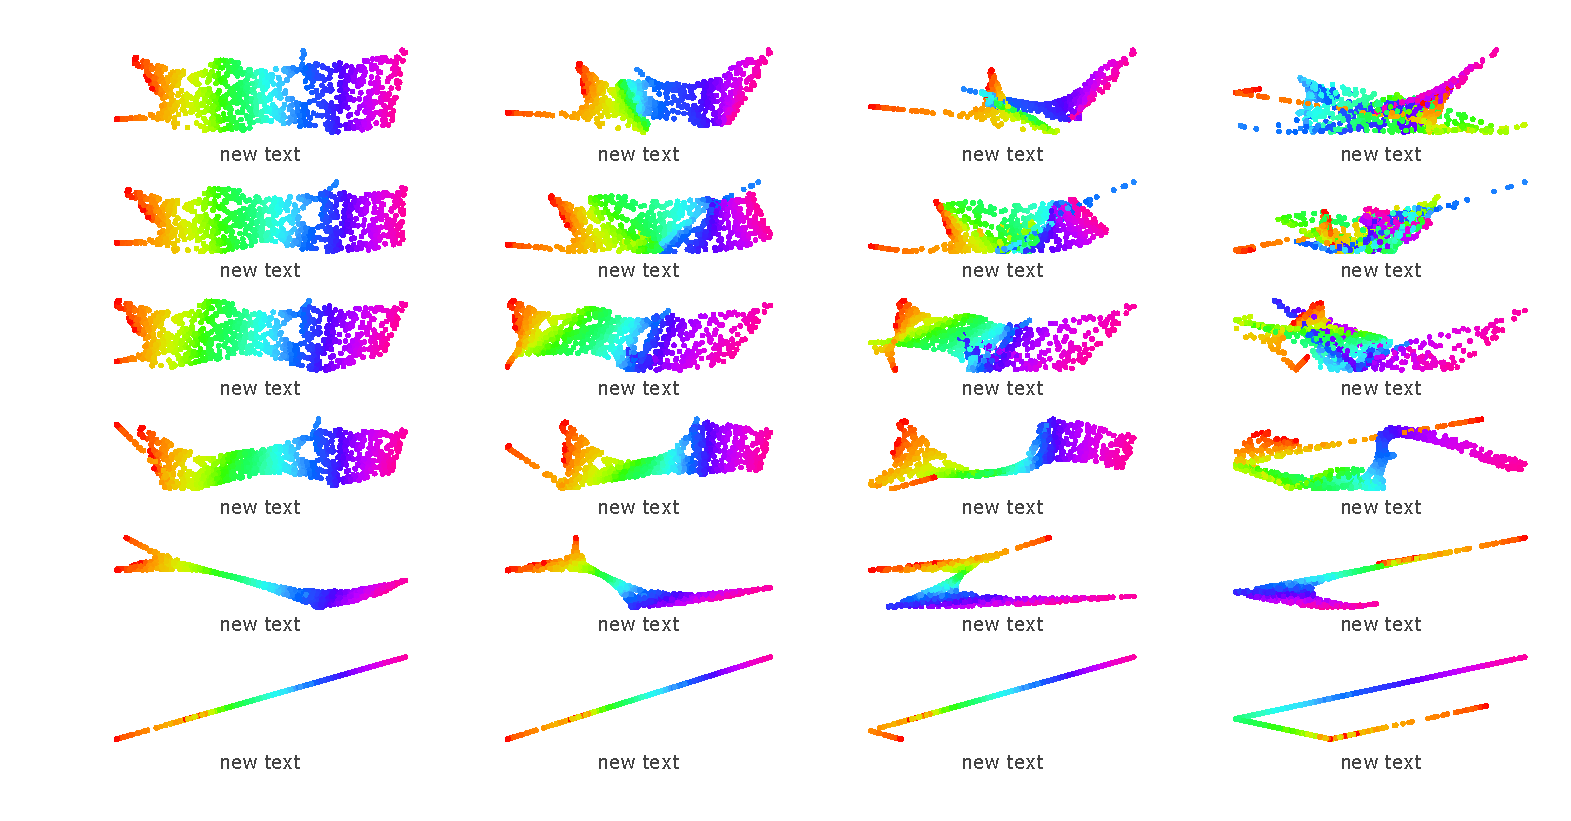
\includegraphics[trim = 40 60 0 0, clip, % left bottom right top
    width = \textwidth]{figures/sensitivity_noise_qual_swiss_roll}

\end{frame}

% ------------------------------------------------------------------------------

\LARGE
\begin{frame}{\textcolor{gray!90}{4.2 results} ~~ sensitivity analysis II}
\normalsize
\vspace{-0.5cm}
\noindent \textcolor{gray!90}{\rule{\textwidth}{1pt}}
\smallskip

\textbf{Qualitative results:} incomplete tire

\vspace{0.3cm}

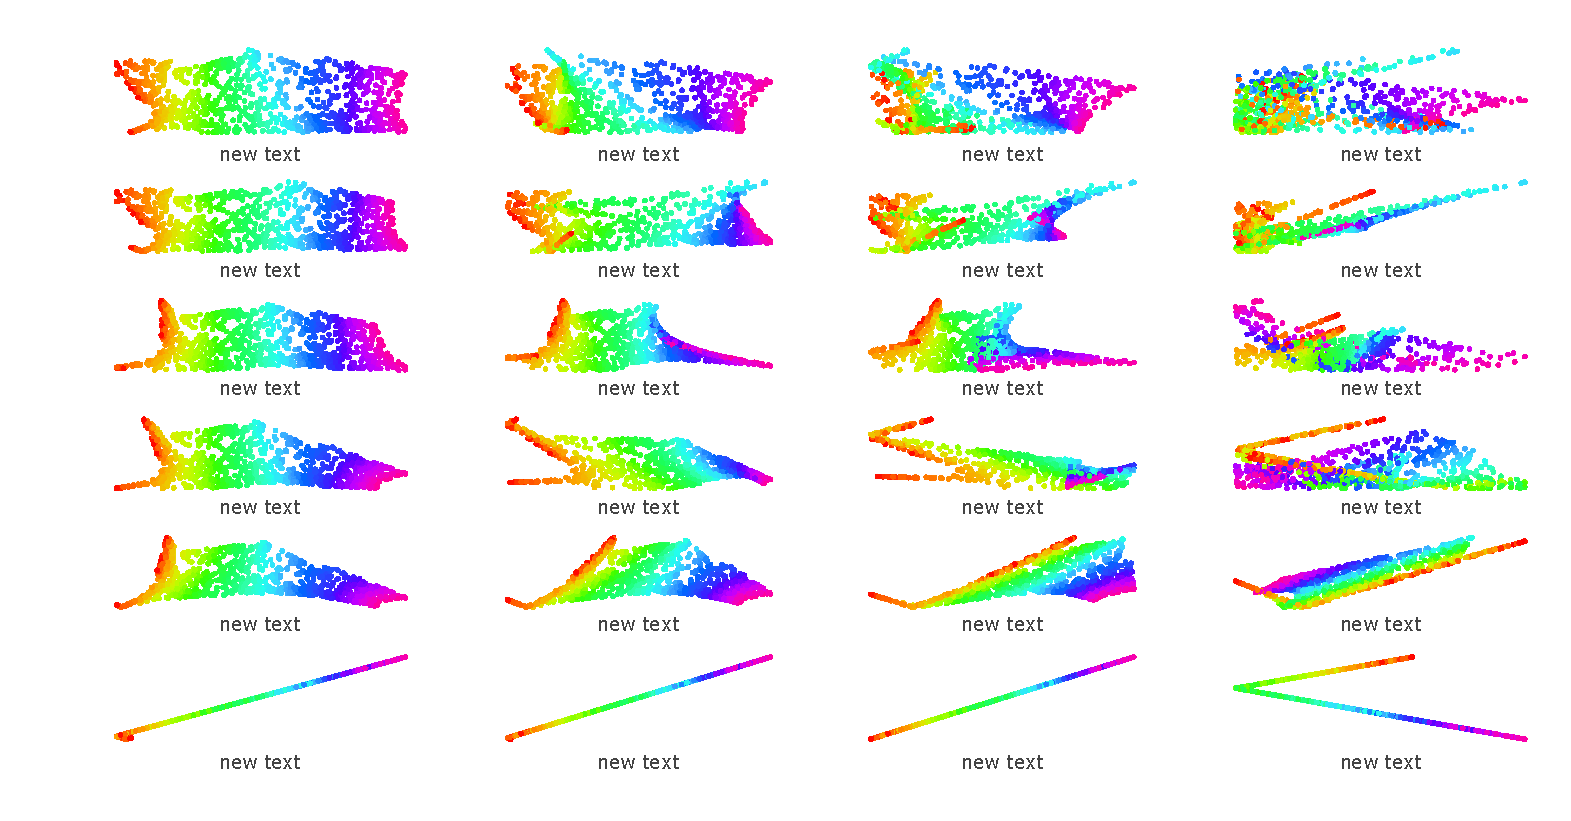
\includegraphics[trim = 40 60 0 0, clip, % left bottom right top
    width = \textwidth]{figures/sensitivity_noise_qual_incomplete_tire}

\end{frame}

% ------------------------------------------------------------------------------

\LARGE
\begin{frame}{\textcolor{gray!90}{4.2 results} ~~ concluding comparison}
\normalsize
\vspace{-0.5cm}
\noindent \textcolor{gray!90}{\rule{\textwidth}{1pt}}
\smallskip

\textbf{Comparison:} LLE vs HLLE vs SSLLE

\vspace{0.3cm}

\begin{minipage}[c]{0.2\textwidth}
  Swiss roll
\end{minipage}%
\begin{minipage}[c]{0.8\textwidth}
  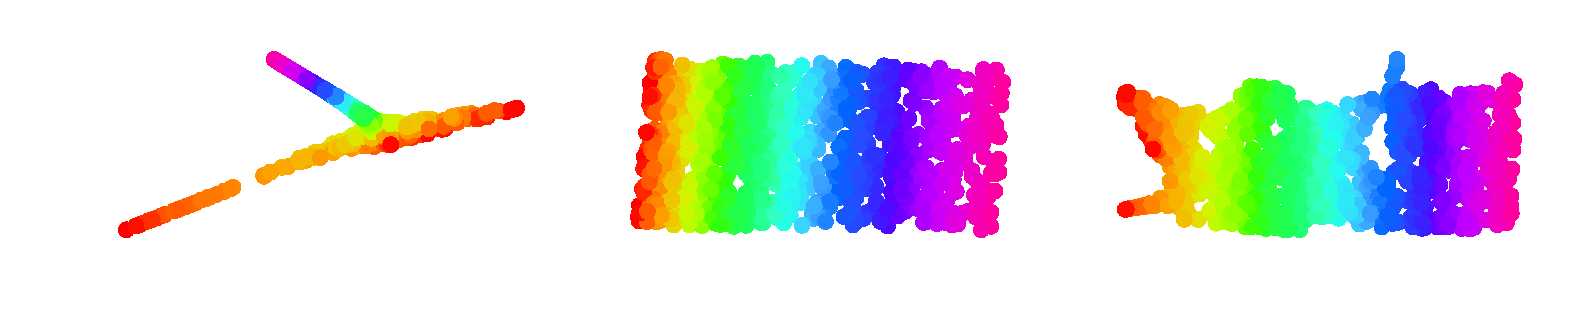
\includegraphics[trim = 0 0 0 0, clip, % left bottom right top
    width = \textwidth]{figures/comparison_swiss_roll}
\end{minipage}

\vspace{0.3cm}   

\begin{minipage}[c]{0.2\textwidth}
  Incomplete tire
\end{minipage}%
\begin{minipage}[c]{0.8\textwidth}
  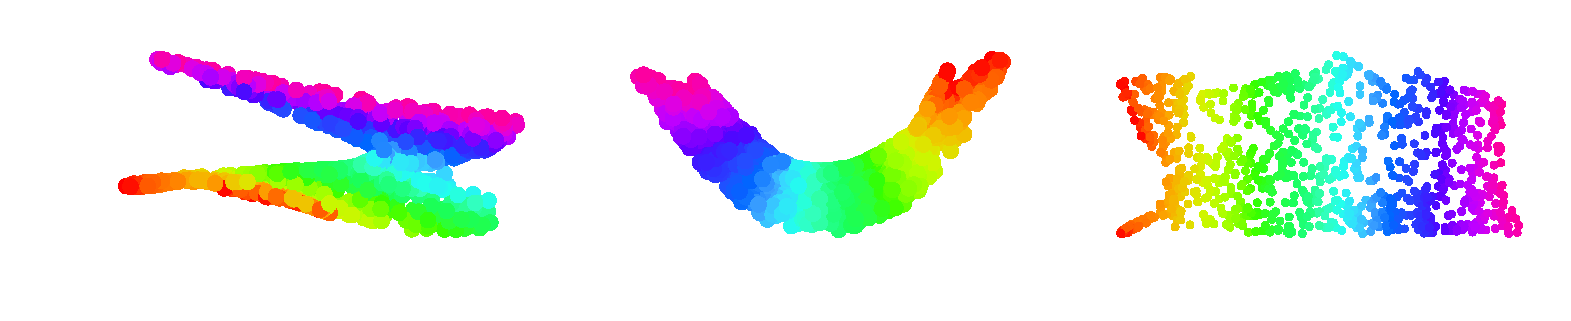
\includegraphics[trim = 0 0 0 0, clip, % left bottom right top
    width = \textwidth]{figures/comparison_incomplete_tire}
\end{minipage}

% \begin{minipage}[b]{0.5\textwidth}
%   \raggedright
%   \textbf{Swiss roll}. LLE, HLLE, SSLLE
%   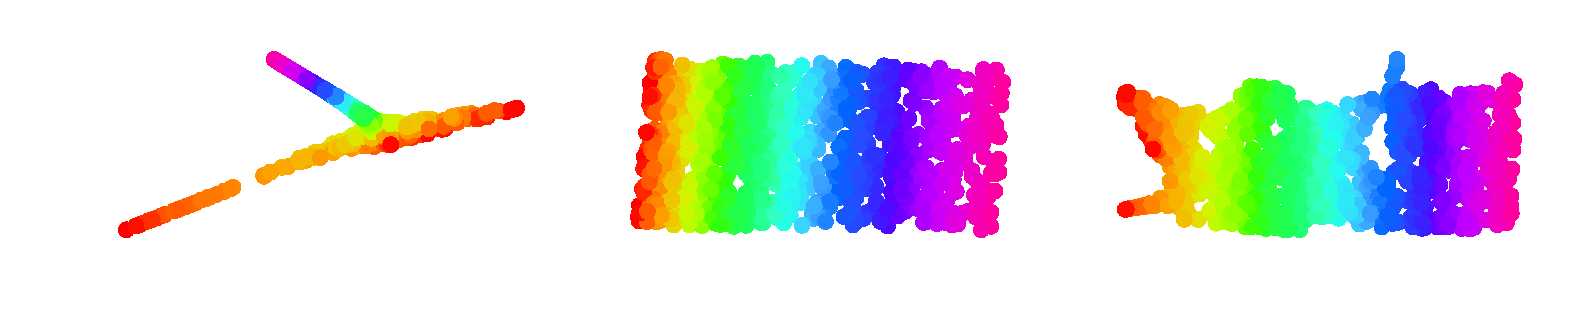
\includegraphics[trim = 0 0 0 0, clip, % left bottom right top
%     width = 0.7\textwidth]{figures/comparison_swiss}
% \end{minipage}%
% \begin{minipage}[b]{0.5\textwidth}
%   \raggedright
%   \textbf{Incomplete tire}. LLE, HLLE, SSLLE
%   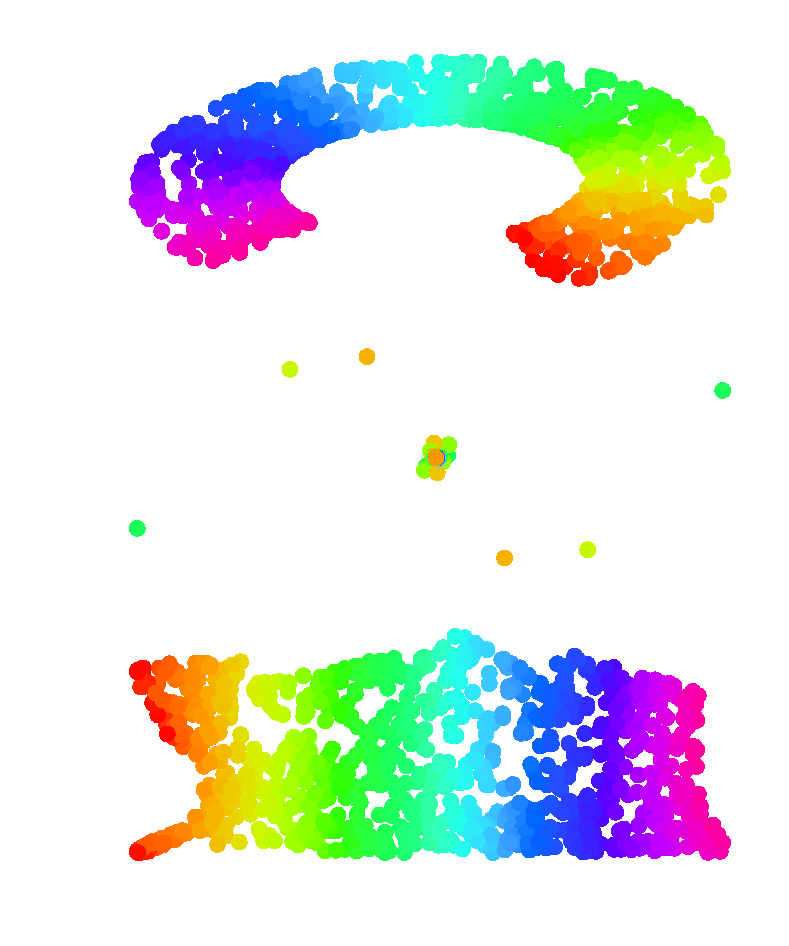
\includegraphics[trim = 0 0 0 0, clip, % left bottom right top
%     width = 0.7\textwidth]{figures/comparison_tire}
% \end{minipage}

\vspace{0.3cm}  

\scriptsize
SSLLE: own implementation (see 
\href{https://github.com/lisa-wm/manifold-lle/tree/main/2_code}{Github}), 
LLE \& HLLE: implementation in \texttt{R}'s \texttt{dimRed} 
package \citep{pkgdimred}. \\
SSLLE with maximum coverage, 12 landmarks and exact prior information,
LLE and HLLE with number of neighbors as deemed optimal by SSLLE implementation 
(no other hyperparameters to set).

\end{frame}

% ------------------------------------------------------------------------------
% DISCUSSION
% ------------------------------------------------------------------------------

\LARGE
\begin{frame}[noframenumbering]{\phantom{foo}}
\normalsize
\vspace{-0.5cm}
\noindent \textcolor{gray!90}{\rule{\textwidth}{1pt}}
\smallskip

\Huge
\hspace{0pt}
\vfill
\textbf{\highlight{~~ 5 ~~ DISCUSSION}}
\vfill
\hspace{0pt}

\noindent \textcolor{gray!90}{\rule{\textwidth}{1pt}}

\end{frame}

% ------------------------------------------------------------------------------

\LARGE
\begin{frame}{\textcolor{gray!90}{5 discussion}}
\normalsize
\vspace{-0.5cm}
\noindent \textcolor{gray!90}{\rule{\textwidth}{1pt}}
\smallskip

% \textbf{Sensitivity.} 

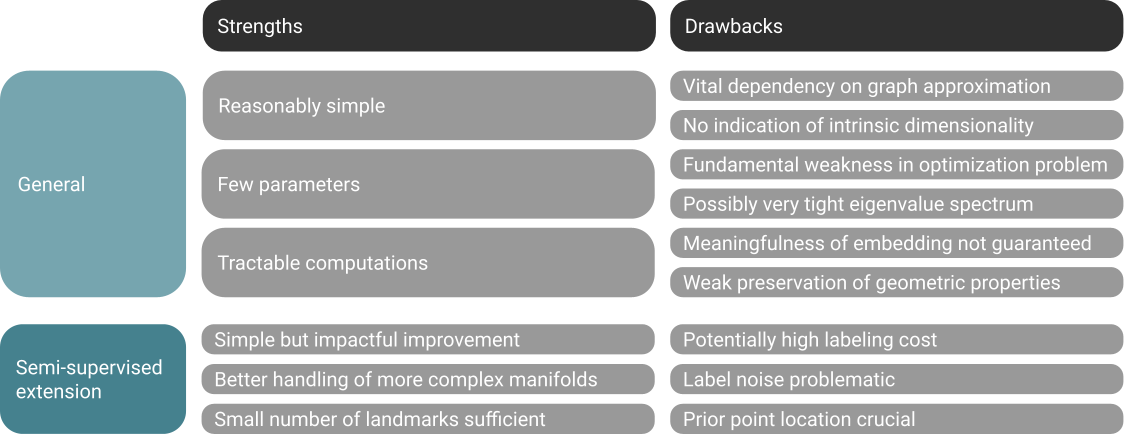
\includegraphics[trim = 0 0 0 0, clip, % left bottom right top
    width = \textwidth]{figures/discussion}
    
\vfill

\conclbox{SSLLE: imperfect but potentially powerful approach to LGML}

\end{frame}

% ------------------------------------------------------------------------------
% APPENDIX
% ------------------------------------------------------------------------------

\LARGE
\begin{frame}[noframenumbering]{\phantom{foo}}
\normalsize
\vspace{-0.5cm}
\noindent \textcolor{gray!90}{\rule{\textwidth}{1pt}}
\smallskip

\Huge
\hspace{0pt}
\vfill
\textbf{\highlight{~~ APPENDIX}}
\vfill
\hspace{0pt}

\noindent \textcolor{gray!90}{\rule{\textwidth}{1pt}}

\end{frame}

% ------------------------------------------------------------------------------

\LARGE
\begin{frame}[noframenumbering]{application to world data set}
\normalsize
\vspace{-0.5cm}
\noindent \textcolor{gray!90}{\rule{\textwidth}{1pt}}
\smallskip

\textbf{Original:} world data in 3D and true 2D embedding 

\begin{minipage}[c]{0.4\textwidth}
  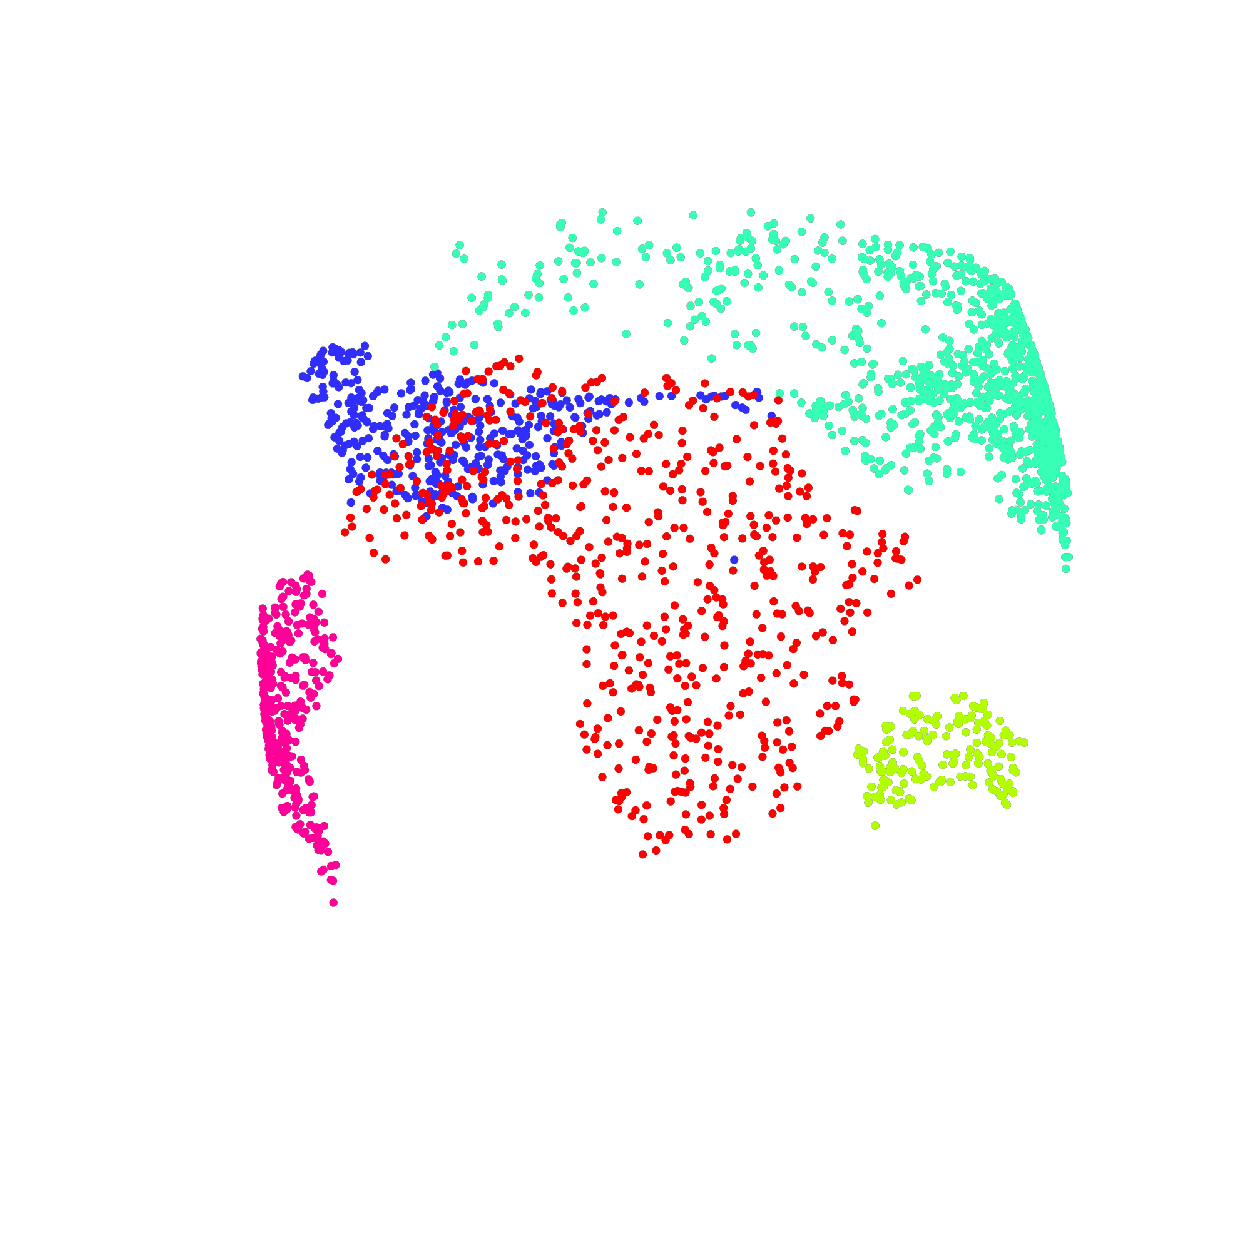
\includegraphics[trim = 0 0 0 0, clip, % left bottom right top
      width = \textwidth]{figures/world_3d}
\end{minipage}%
\begin{minipage}[c]{0.6\textwidth}
  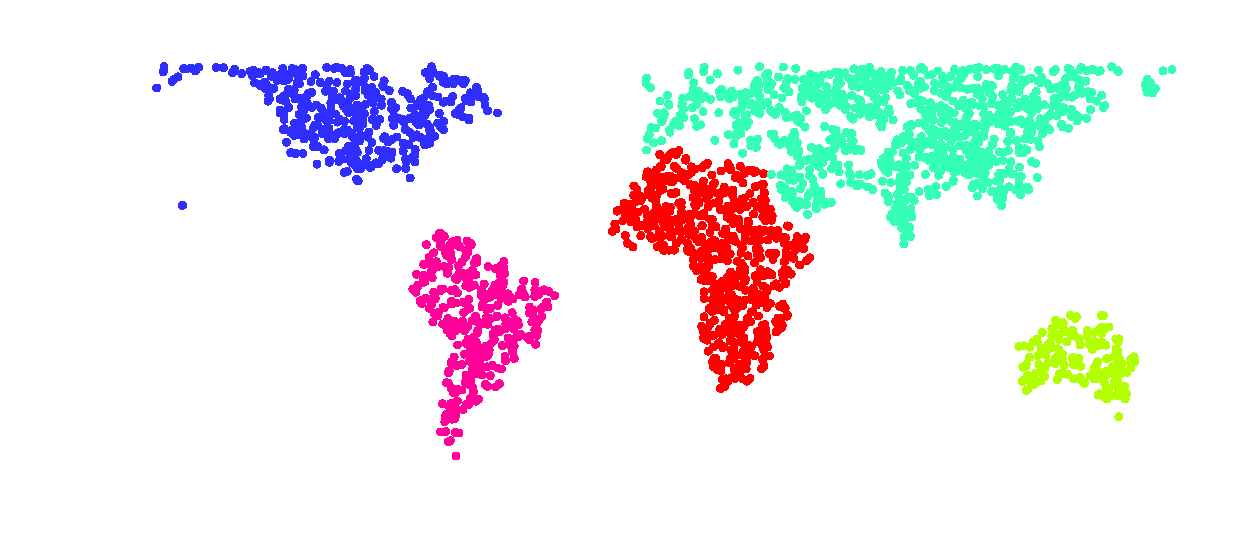
\includegraphics[trim = 0 0 0 50, clip, % left bottom right top
      width = \textwidth]{figures/world_2d}
\end{minipage}

\end{frame}

% ------------------------------------------------------------------------------
% BIBLIOGRAPHY
% ------------------------------------------------------------------------------

\LARGE
\begin{frame}[noframenumbering]{\phantom{foo}}
\normalsize
\vspace{-0.5cm}
\noindent \textcolor{gray!90}{\rule{\textwidth}{1pt}}
\smallskip

\Huge
\hspace{0pt}
\vfill
\textbf{\highlight{~~ MAIN REFERENCES}}
\vfill
\hspace{0pt}

\noindent \textcolor{gray!90}{\rule{\textwidth}{1pt}}

\end{frame}

% ------------------------------------------------------------------------------

\begin{frame}<presentation:0>[noframenumbering]

\citep{bengioetal2004}
\citep{ghojoghetal2020}
\citep{cayton2005}
\citep{vandermaatenetal2009}
\citep{sauletal2006}

\end{frame}

% ------------------------------------------------------------------------------

\begin{frame}[noframenumbering]{}
\scriptsize

\bibliography{bibliography}
\bibliographystyle{dcu}

\end{frame}

% ------------------------------------------------------------------------------

\endlecture

\end{document}